\documentclass[a4paper, 12pt]{article}%тип документа

%отступы
\usepackage[left=2cm,right=2cm,top=2cm,bottom=3cm,bindingoffset=0cm]{geometry}

%Русский язык
\usepackage[T2A]{fontenc} %кодировка
\usepackage[utf8]{inputenc} %кодировка исходного кода
\usepackage[english,russian]{babel} %локализация и переносы

%Вставка картинок
\usepackage{wrapfig}
\usepackage{graphicx}
\graphicspath{{pictures/}}
\DeclareGraphicsExtensions{.pdf,.png,.jpg}

%оглавление
\usepackage{titlesec}
\titlespacing{\chapter}{0pt}{-30pt}{12pt}
\titlespacing{\section}{\parindent}{5mm}{5mm}
\titlespacing{\subsection}{\parindent}{5mm}{5mm}
\usepackage{setspace}

%Графики
\usepackage{multirow}
\usepackage{pgfplots}
\pgfplotsset{compat=1.9}

%Математика
\usepackage{amsmath, amsfonts, amssymb, amsthm, mathtools}

\begin{document}

\begin{titlepage}

\begin{center}
%\vspace*{1cm}
\large\textbf{Московский Физико-Технический Институт}\\
\large\textbf{(государственный университет)}
\vfill
\line(1,0){430}\\[1mm]
\huge\textbf{Работа 23}\\
\line(1,0){430}\\[1mm]
\vfill
\large Сибгатуллин Булат, ФРКТ\\
\end{center}

\end{titlepage}

\section*{ЗАДАНИЕ 1}

\begin{enumerate}

\item Зарисуем схему цепи.

\begin{figure}[h!]
\centering
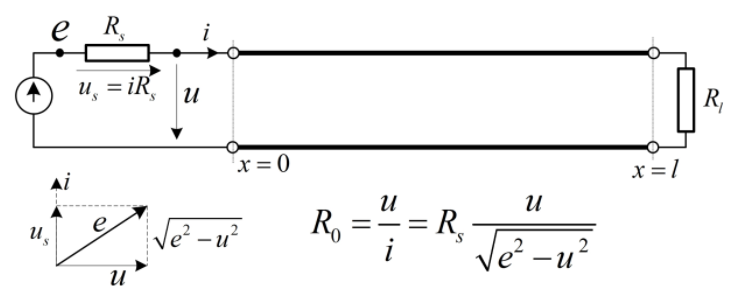
\includegraphics[scale=1]{images/Scheme1.png}
\label{fig:Image1}
\end{figure}

\item Измерим длину \textit{l} кабеля:

\[l \simeq 5,82 \: \textit{м}\]

Запишем параметры цепи:

\[R_{s1} = 36,4 \: (36) \: \textit{Ом}\]

\[R_{s2} = 441 \: (430) \: \textit{Ом}\]

\[f = 1,1 \: \textit{МГц}\]

В режиме котороткого замыкания на выходе будем использовать резистор $R_{s1}$, а в режиме холостого хода на выходе будем использовать резистор $R_{s2}$. Найдем входное сопротивление линии по формуле:

\[R_0 = R_s \frac{u}{\sqrt{e^2 - u^2}}\]

Для $R_{01}$, $u = 1,48 \: \textit{В}$, а $e = 2,91 \: \textit{В}$. Получаем:

\[R_{01} = 21,54 \: \textit{Ом} \: (\text{Короткое замыкание})\]

Для $R_{02}$, $u = 1,75 \: \textit{В}$, а $e = 3,23 \: \textit{В}$. Получаем:

\[R_{02} = 281 \: \textit{Ом} \: (\text{Холостой ход})\]

\item Вычислим $\omega$ и $v$:

\[\omega = \sqrt{\frac{L}{C}} = \sqrt{R_{01}\cdot R_{02}} = 77,5 \: \textit{Ом}\]

\[v = \frac{1}{\sqrt{LC}} \simeq 2 \pi f l \frac{\omega}{R_{01}} = 1,7 \cdot 10^8 \: \textit{м/с}\]

Оценим погонные емкость $C$ и индуктивность $L$:

\[C = \frac{1}{\omega v} = 7,59 \cdot 10^{-11} \: \textit{Ф}\]

\[L = \frac{\omega}{v} = 4,56 \cdot 10^{-7} \: \textit{Гн}\]

\item Исследуем резонансный пик на частоте $f_0 = 7,5 \: \textit{МГц}$ и $R_s = 980 \: (1000) \: \textit{Ом}$. Получим:

\[u = 2,44 \: \textit{В}, \quad e = 3,78 \: \textit{В}\]

\[\frac{1}{\sqrt{2}} \frac{u}{e} = 0,45,\]

Это уровень по которому мы ищем значения частоты для ширины полочу пропускания.

\[f_1 = 6,5 \: \textit{МГц}, \quad f_2 = 8,5 \: \textit{МГц}\]

\[\bigtriangleup f = 2 \: \textit{МГц}\]

\[R_0 = 1748 \: \textit{Ом}\]

\item Вычислим погонное сопротивление линии:

\[R = \frac{\omega^2}{R_0 l} = 0,59 \: \textit{Ом}\]

Вычислим добротность по формуле:

\[Q = \frac{f_0}{\bigtriangleup f} \Big(1 + \frac{R_0}{R_s}\Big) = 21\]

Что близко к ожидаемому значению:

\[Q = \frac{\pi}{4} \frac{\omega}{Rl} = 18\]

\end{enumerate}

\section*{ЗАДАНИЕ 2}

\subsection*{Согласованная линия} Откроем файл \textbf{TLine.cir}. Зарисуем схему.

\begin{figure}[h!]
\centering
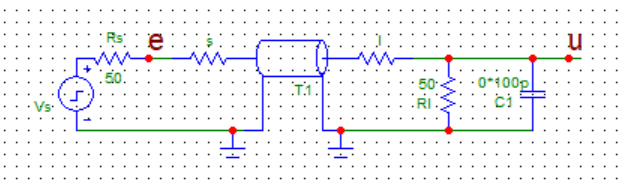
\includegraphics[scale=1]{images/TLine.png}
\label{fig:Image1}
\end{figure}

На схеме установим $R_s = R_l = 50$ Ом и выведем график в режиме \textit{Transient}.

\begin{figure}[h!]
\centering
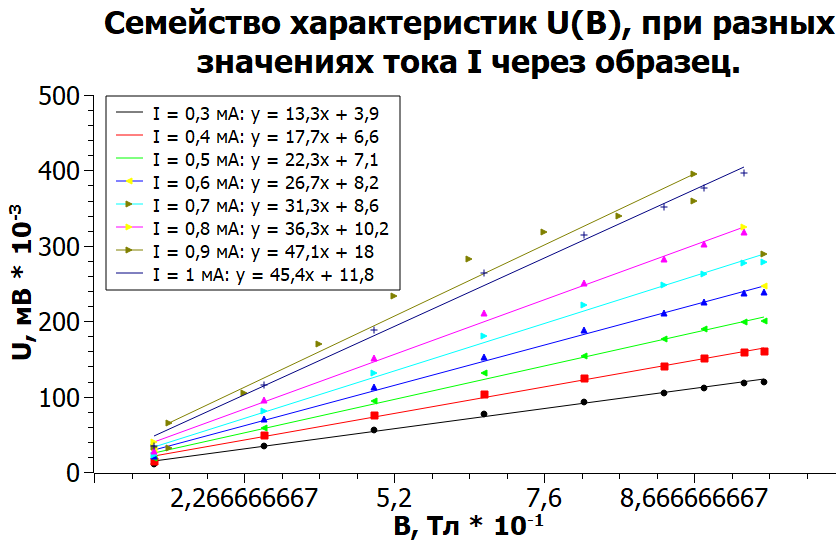
\includegraphics[scale=0.4]{images/Graph1.png}
\label{fig:Image1}
\end{figure}

Проанализируем графики и получим: $u(v) = 0,5 \: \textit{В}$ и $i(l)\cdot \omega = 0,5 \: \textit{В}$. Убедимся, что источник отражает предельную мощность:

\[P = v(u)i(l) = \frac{V^2}{4R_s}, \: \text{где} \: V = 1\textit{В}\]

\[P\omega = v(u)i(l)\omega = 0,5\cdot 0,5 = 0,25 = \frac{V^2}{4R_s} \omega,\]

убедились, что источник отражает предельную мощность.

\subsection*{Рассогласованный источник}

Установим $R_s = \frac{\omega}{3} = \frac{50}{3} \: \textit{Ом}$. Выведем график в режиме \textit{Transient}.

\begin{figure}[h!]
\centering
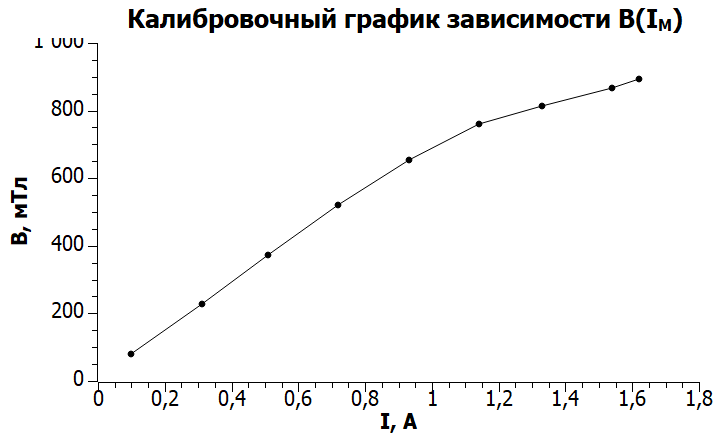
\includegraphics[scale=0.4]{images/Graph2.png}
\label{fig:Image1}
\end{figure}

Проанализируем графики и получим: $u(v) = 0,75 \: \textit{В}$ и $i(l)\cdot \omega = 0,75 \: \textit{В}$. Проверим, что отдаваемая мощность \textit{P} меньше мощности источника в $(1 - \rho_s^2$ раз:

\[\rho_s = \frac{R_s - \omega}{R_s + \omega} = -\frac{1}{2}\]

\[P\omega = v(u)i(l)\omega = 0,75 \cdot 0,75 = 0,5625 = \frac{V^2}{4R_s} \omega (1 - \rho_s^2),\]

Повторим все это при $R_s = 3\omega = 150 \: \textit{Ом}$

\begin{figure}[h!]
\centering
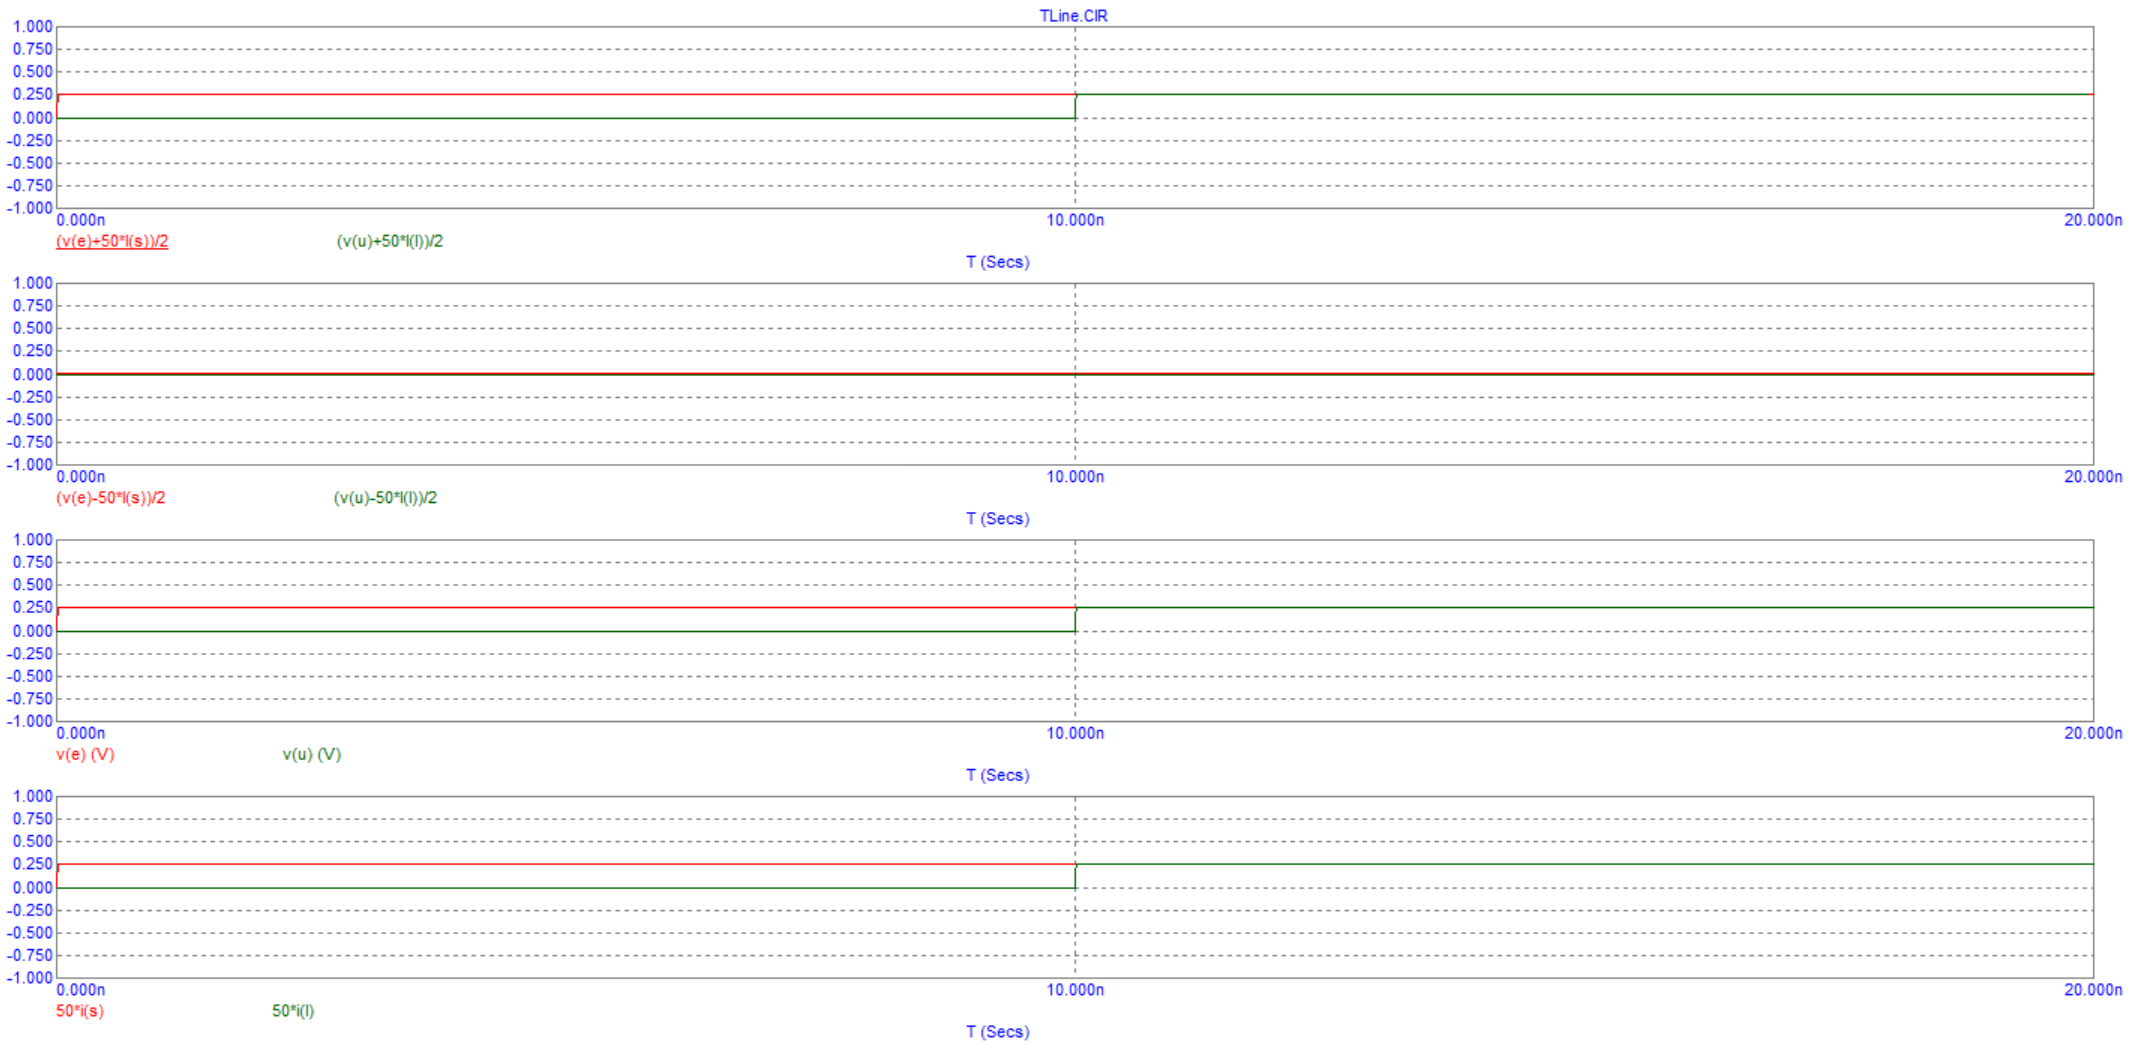
\includegraphics[scale=0.4]{images/Graph3.png}
\label{fig:Image1}
\end{figure}

Проанализируем графики и получим: $u(v) = 0,25 \: \textit{В}$ и $i(l)\cdot \omega = 0,25 \: \textit{В}$. Проверим, что отдаваемая мощность \textit{P} меньше мощности источника в $(1 - \rho_s^2$ раз:

\[\rho_s = \frac{R_s - \omega}{R_s + \omega} = \frac{1}{2}\]

\[P\omega = v(u)i(l)\omega = 0,25 \cdot 0,25 = 0,0625 = \frac{V^2}{4R_s} \omega (1 - \rho_s^2),\]

\subsection*{Рассогласованная нагрузка}

Установим варьированием $R_l = \frac{\omega}{3} = \frac{50}{3} \: \textit{Ом}$ $[\rho_l = - \frac{1}{2}]$, $R_l = 0 \: \textit{Ом}$ $[\rho_l = 0]$, $R_l = 3\omega = 150 \: \textit{Ом}$, $[\rho_l =  \frac{1}{2}]$ ($R_s = 50 \textit{Ом}$). Измерим установившиеся значения амплитуд волн, напряжений и токов.

\begin{figure}[h!]
\centering
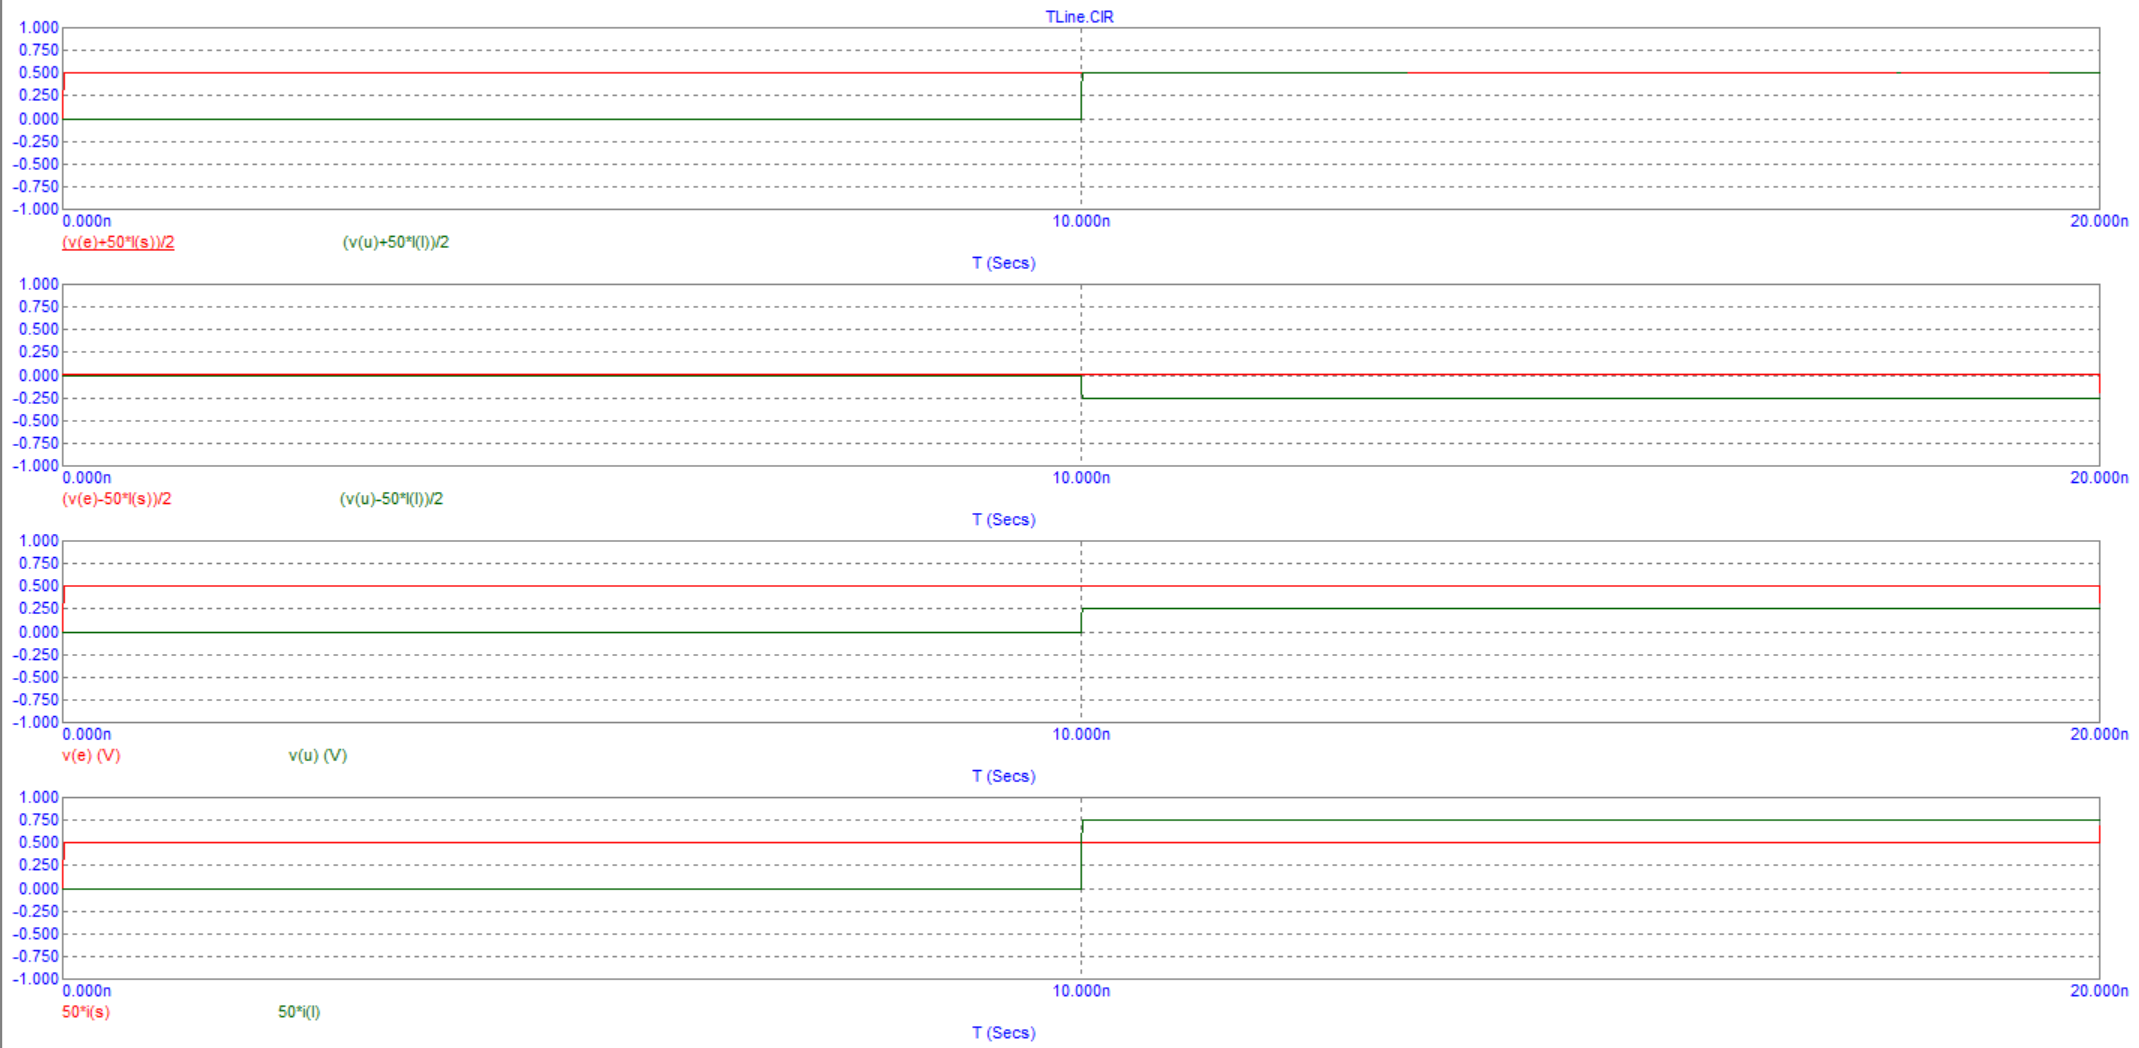
\includegraphics[scale=0.4]{images/Graph4.png}
\label{fig:Image1}
\caption{$R_l = \frac{\omega}{3}$}
\end{figure}

\begin{figure}[h!]
\centering
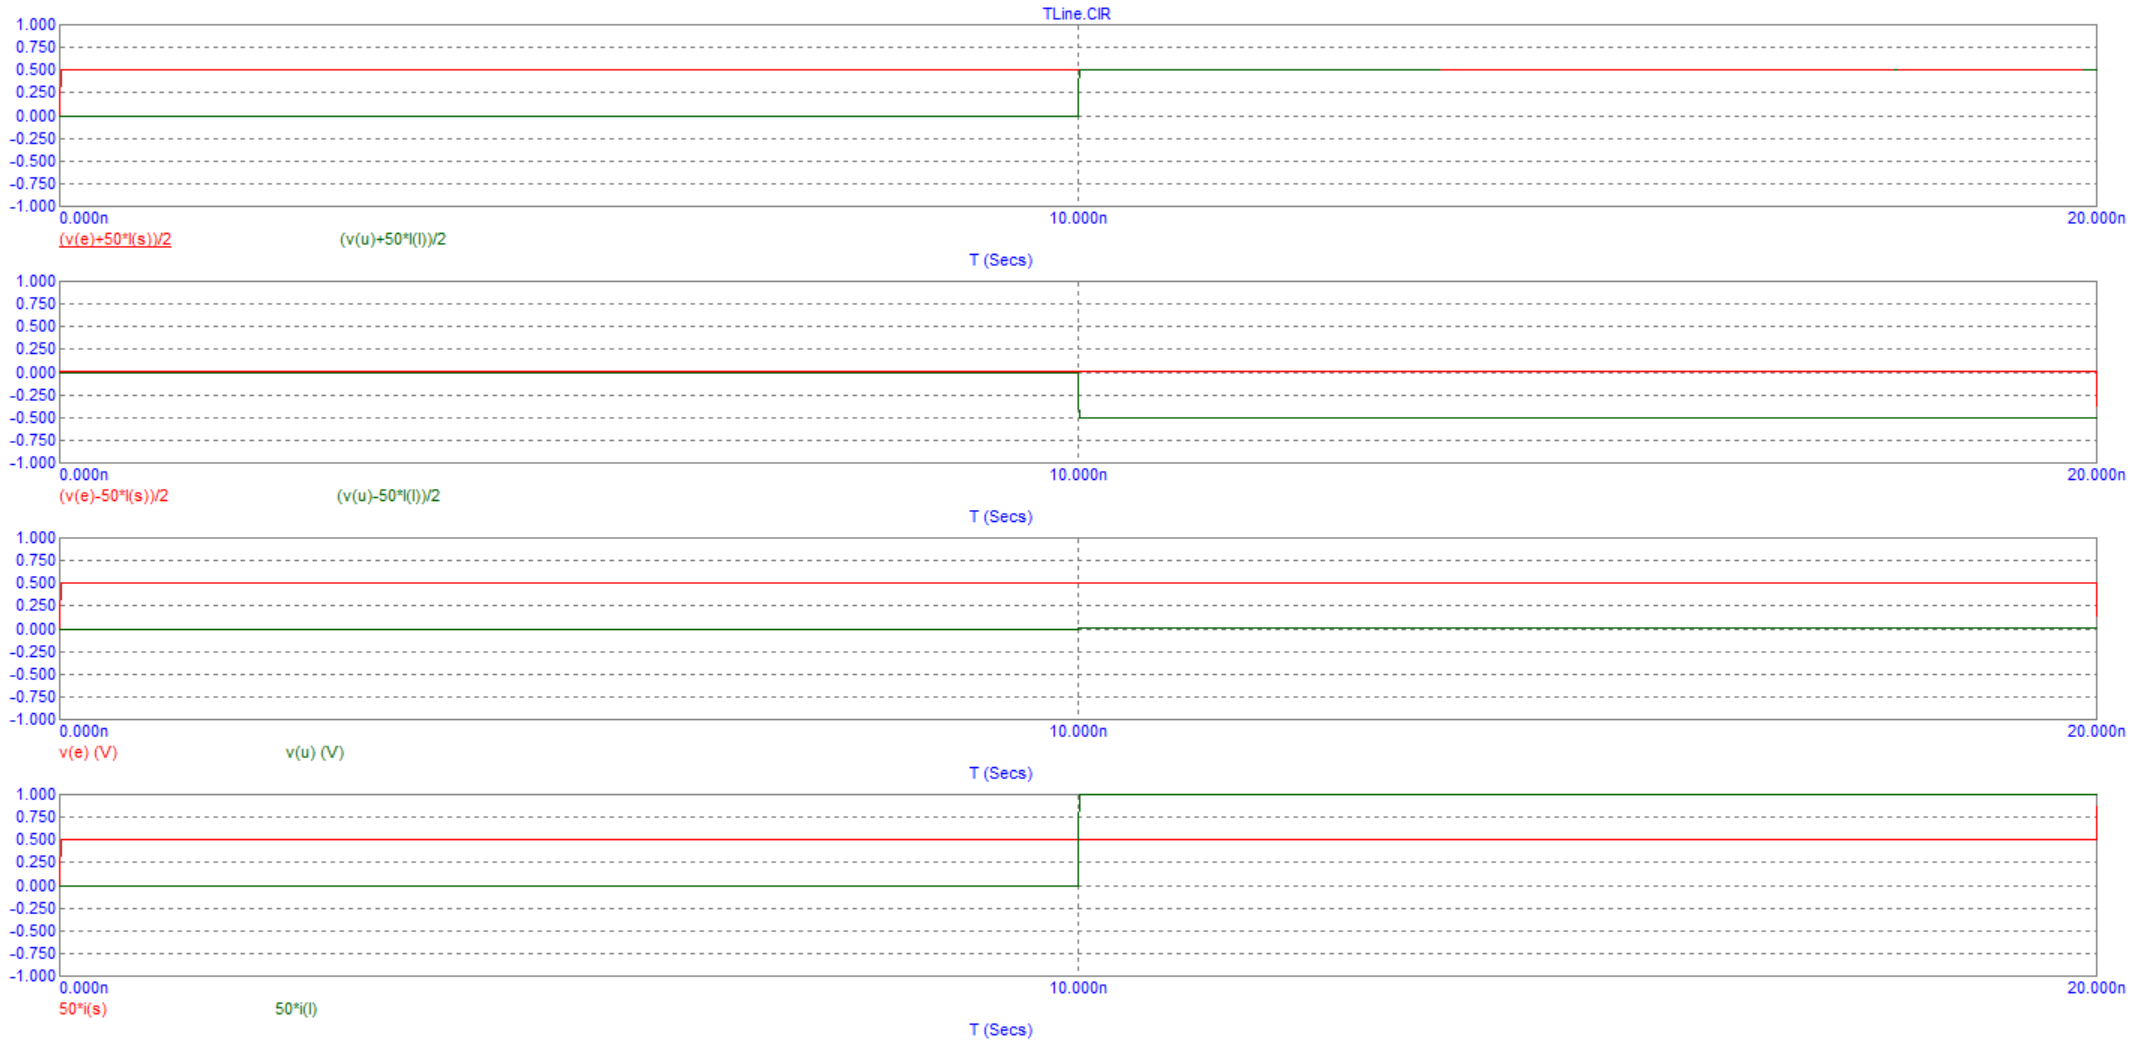
\includegraphics[scale=0.4]{images/Graph5.png}
\label{fig:Image1}
\caption{$R_l = 0$}
\end{figure}

\begin{figure}[h!]
\centering
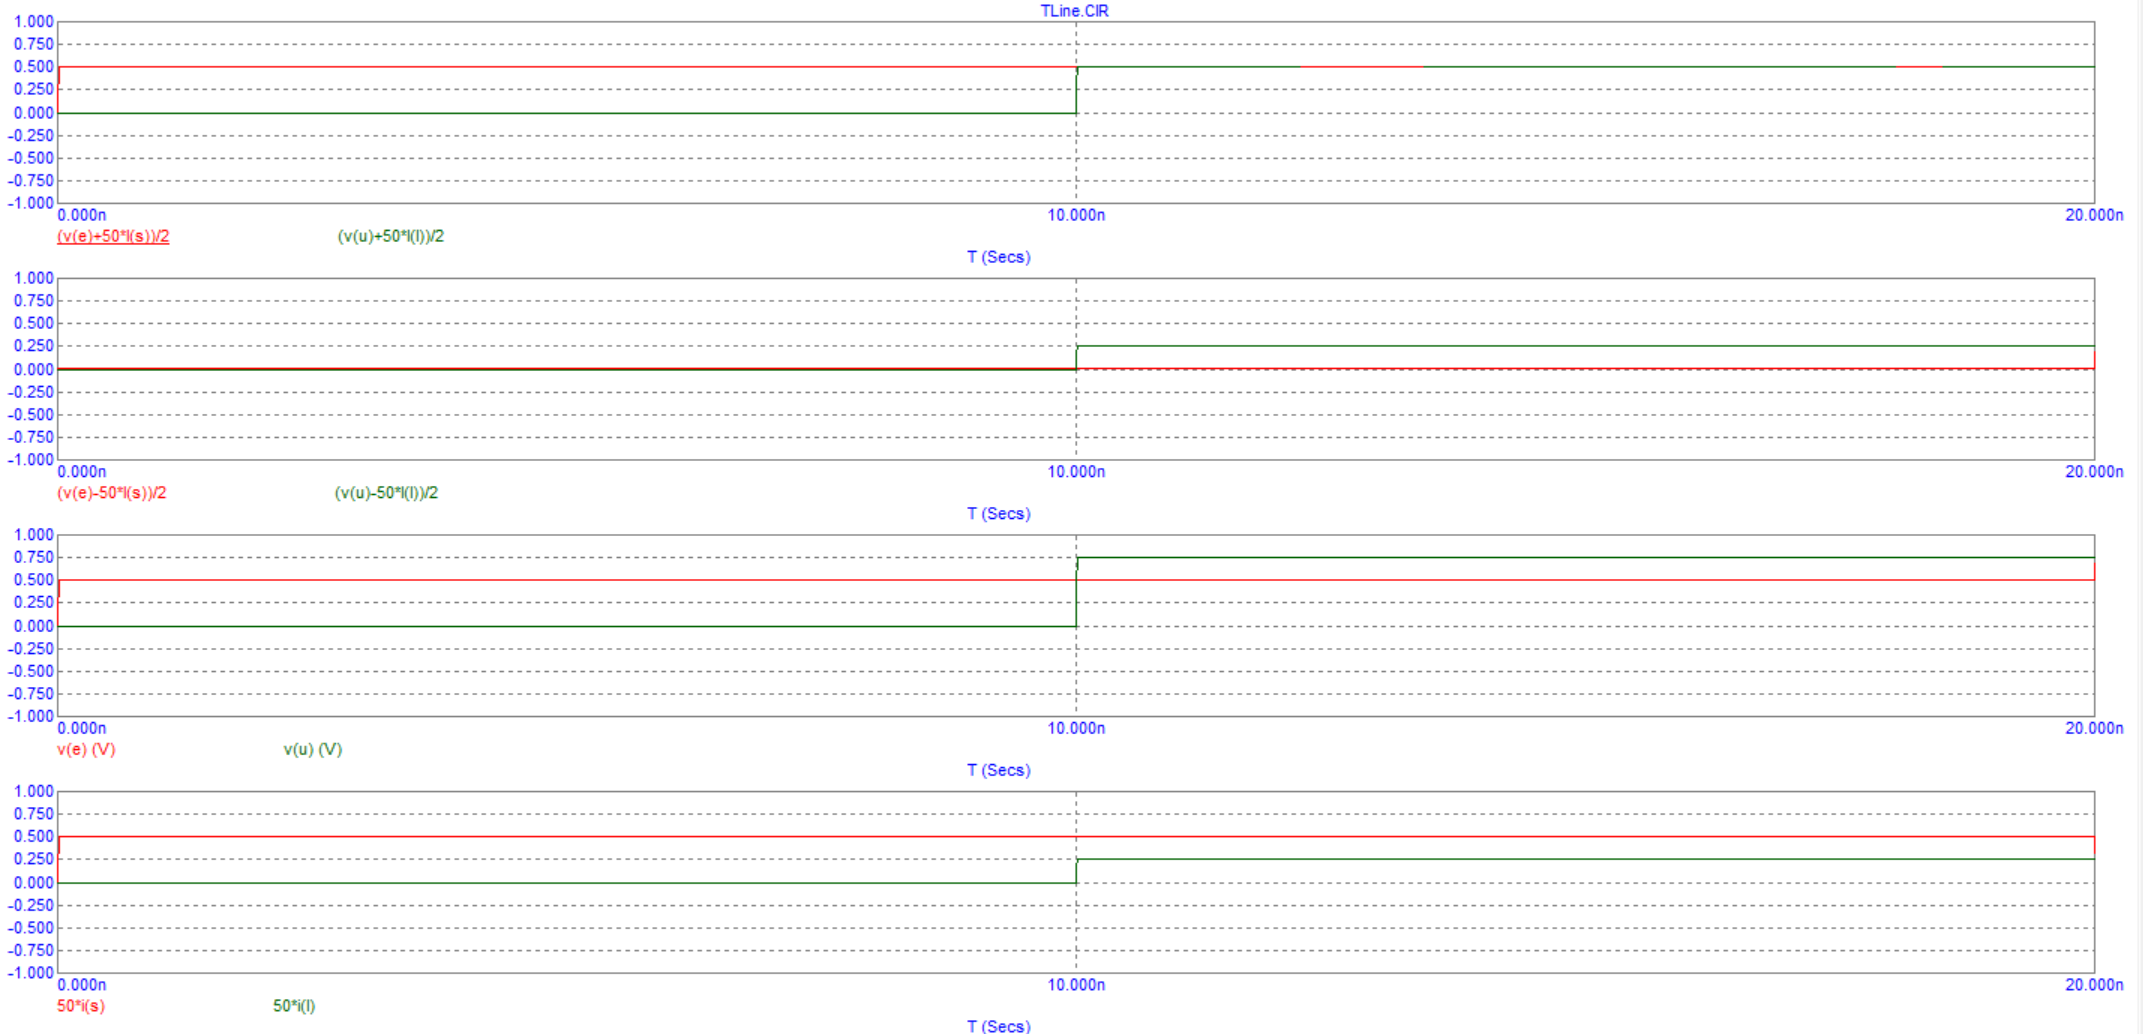
\includegraphics[scale=0.4]{images/Graph6.png}
\label{fig:Image1}
\caption{$R_l = 3\omega$}
\end{figure}

\begin{figure}[h!]
\centering
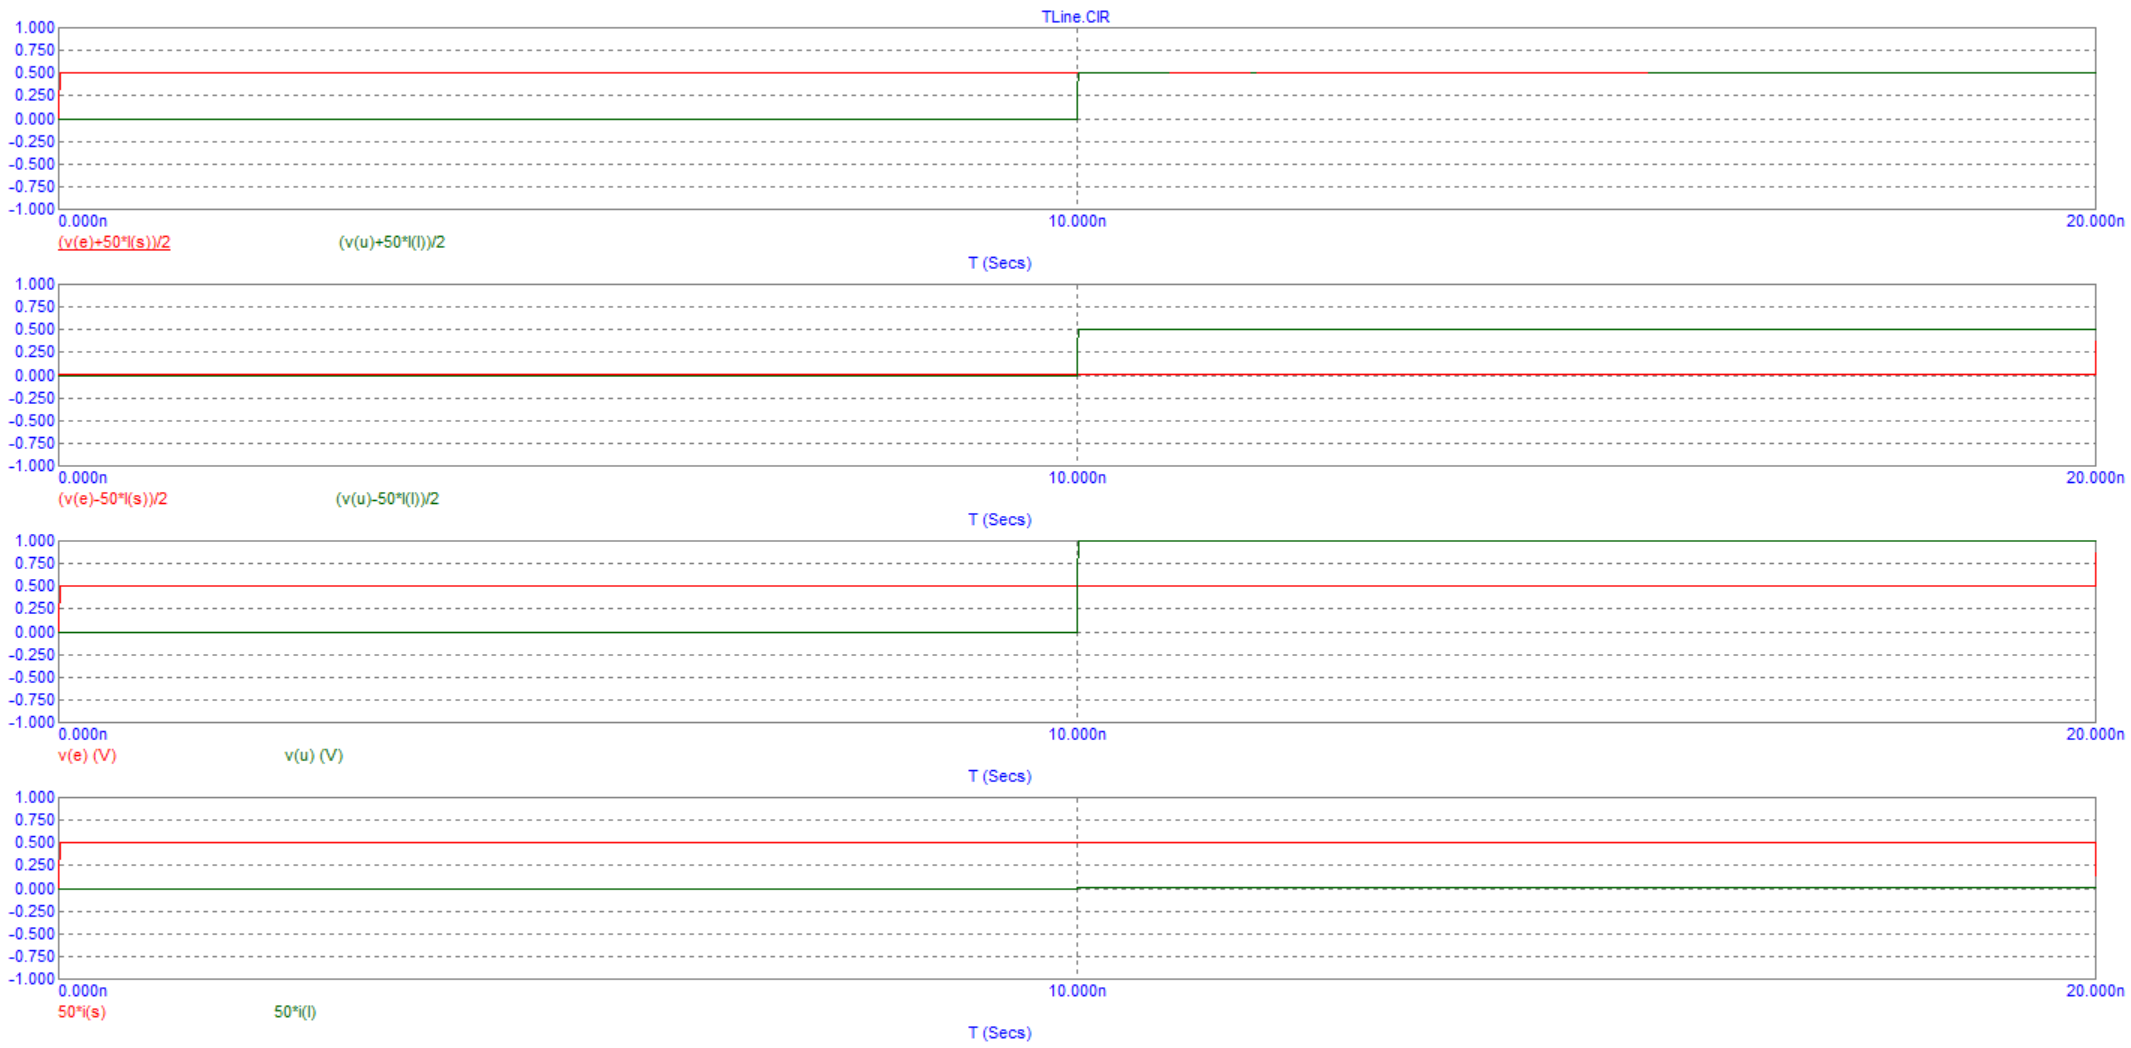
\includegraphics[scale=0.4]{images/Graph7.png}
\label{fig:Image1}
\caption{$R_l = 50k$}
\end{figure}

Запишем данные в таблицу:

\begin{center}
\begin{tabular}{|c|c|c|c|c|}
\hline 
$R_l/\omega$ & 1/3 & 0 & 3 & 50k \\ 
\hline 
A & 0,5 & 0,5 & 0,5 & 0,5 \\ 
\hline 
B & -0,25 & -0,5 & 0,25 & 0,5 \\ 
\hline 
$v(u)$ & 0,25 & 0 & 0,75 & 1 \\ 
\hline 
$i(l)\omega$ & 0,75 & 1 & 0,25 & 0 \\ 
\hline 
\end{tabular} 
\end{center}

\subsection*{Рассогласованные источник и нагрузка}

Установить на схеме $R_s = 50/3 \: [\rho_s = -\frac{1}{2}]$. Установим варьированием $R_l = 0 \: [\rho_l = -1]$, $\rho_s \rho_l = \frac{1}{2}$, выведем графики.

\begin{figure}[h!]
\centering
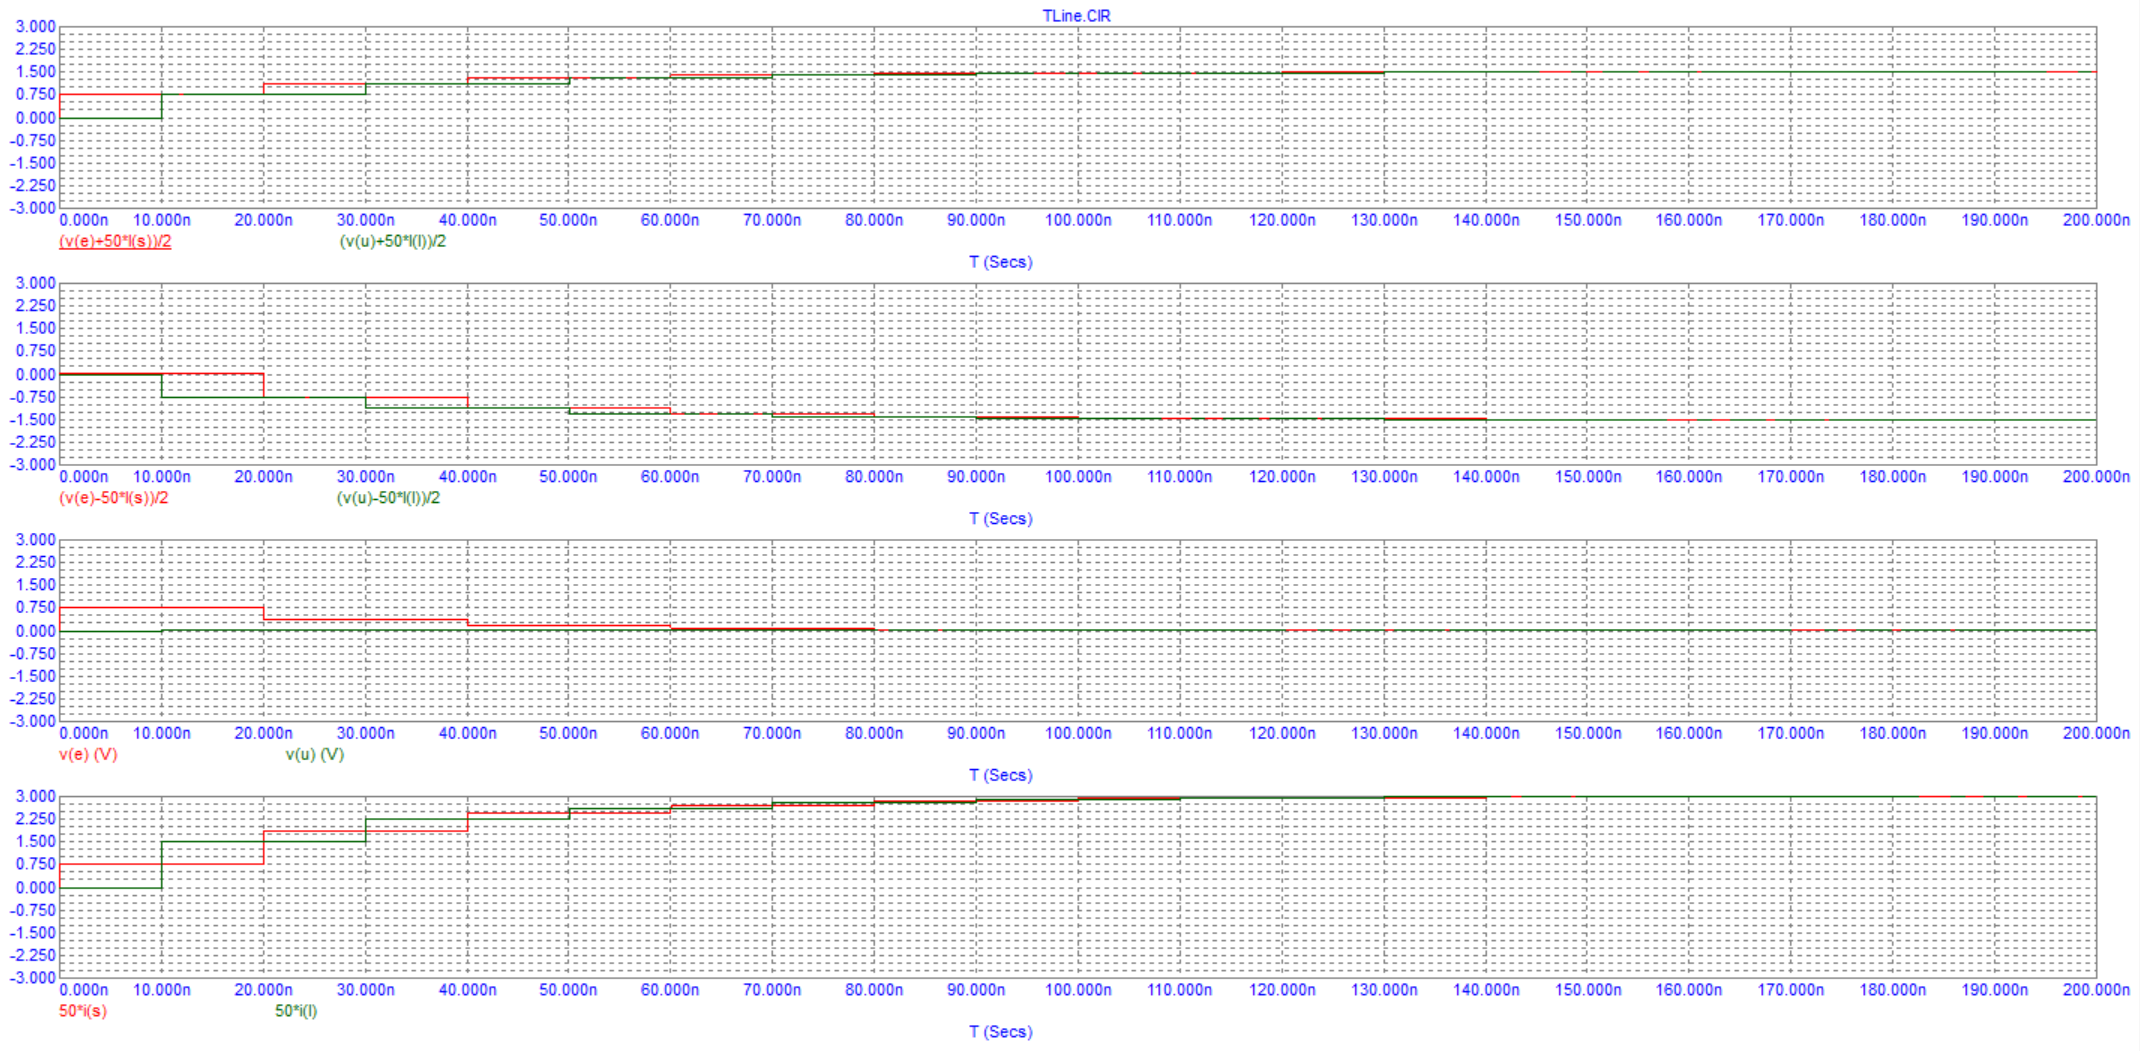
\includegraphics[scale=0.4]{images/Graph8.png}
\label{fig:Image1}
\caption{$R_l = 0, R_s = 50/3$}
\end{figure}

Убедимся в том, что амплитуда пдающей волны нарастает, как последовательных частичных сумм прогрессии:

\[A = \frac{\omega}{\omega + R_s} \Big( 1 + \rho_s \rho_l + (\rho_s \rho_l)^2 + ...\Big) = \frac{3}{4} \Big( 1 + \frac{1}{2} + \frac{1}{4} + ... \Big) = 1,5\]

Первый шаг $(n = 1): \: A = 0,75$.

Второй шаг $(n = 2): \: A = 9/8$.

Третий шаг $(n = 3): \: A = 21/16$.

Установившееся значение: $(n = \infty): \: A = 1,5$.

Повторим наблюдения при $R_l = 50k \simeq \infty \: [\rho_l = 1], \: \rho_s \rho_l = -\frac{1}{2}$:

\begin{figure}[h!]
\centering
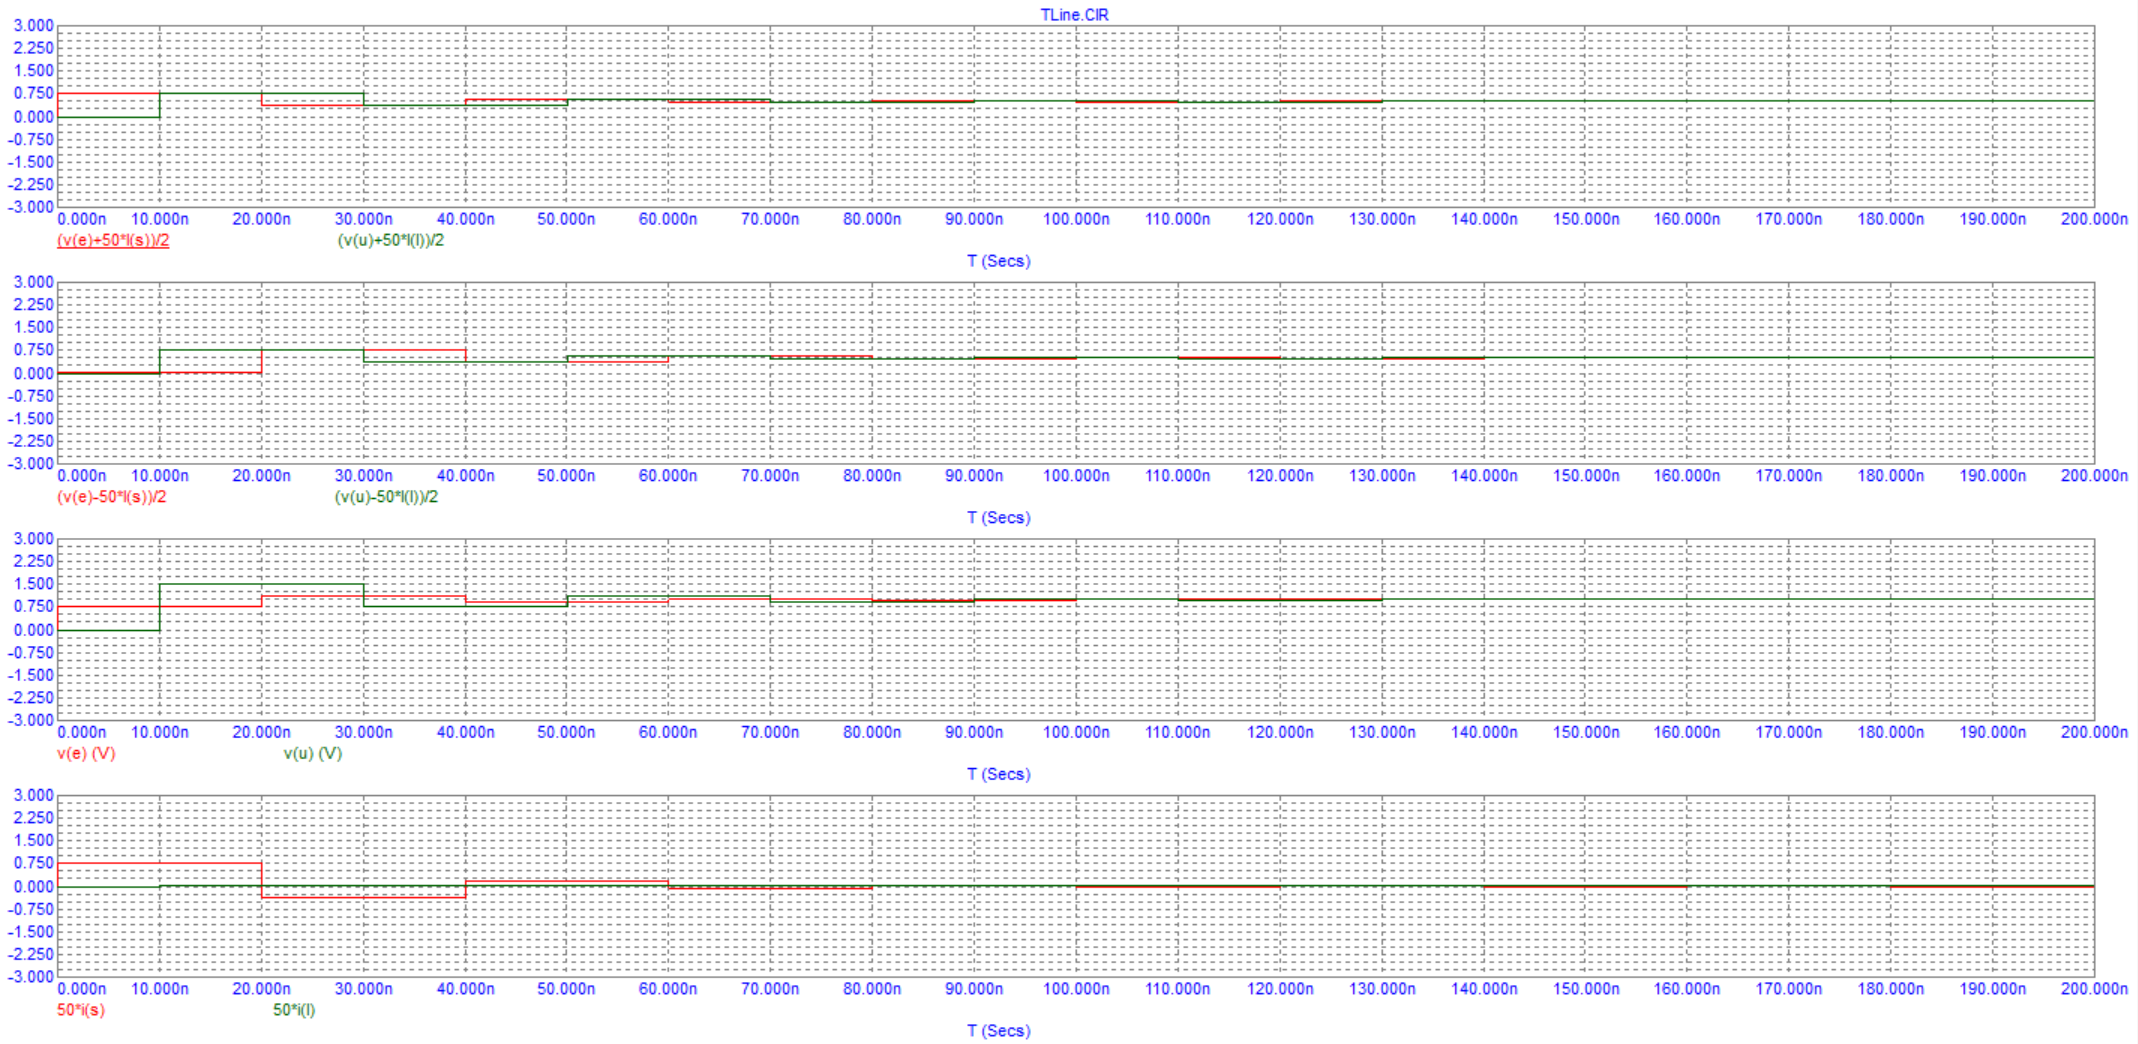
\includegraphics[scale=0.4]{images/Graph9.png}
\label{fig:Image1}
\caption{$R_l = 50k, R_s = 50/3$}
\end{figure}

\[A = \frac{\omega}{\omega + R_s} \Big( 1 + \rho_s \rho_l + (\rho_s \rho_l)^2 + ...\Big) = \frac{3}{4} \Big( 1 - \frac{1}{2} + \frac{1}{4} - ... \Big) = \frac{3}{4} \cdot \frac{2}{3} = \frac{1}{2}\]

Первый шаг $(n = 1): \: A = 0,75$.

Второй шаг $(n = 2): \: A = 3/8$.

Третий шаг $(n = 3): \: A = 9/16$.

Установившееся значение: $(n = \infty): \: A = 0,5$.

Установим на схеме $R_s = 50\omega \: [\rho_s = \frac{1}{2}]$ и повторим наблюдения при $R_l = 0 \:[\rho_l = -1]$.

\begin{figure}[h!]
\centering
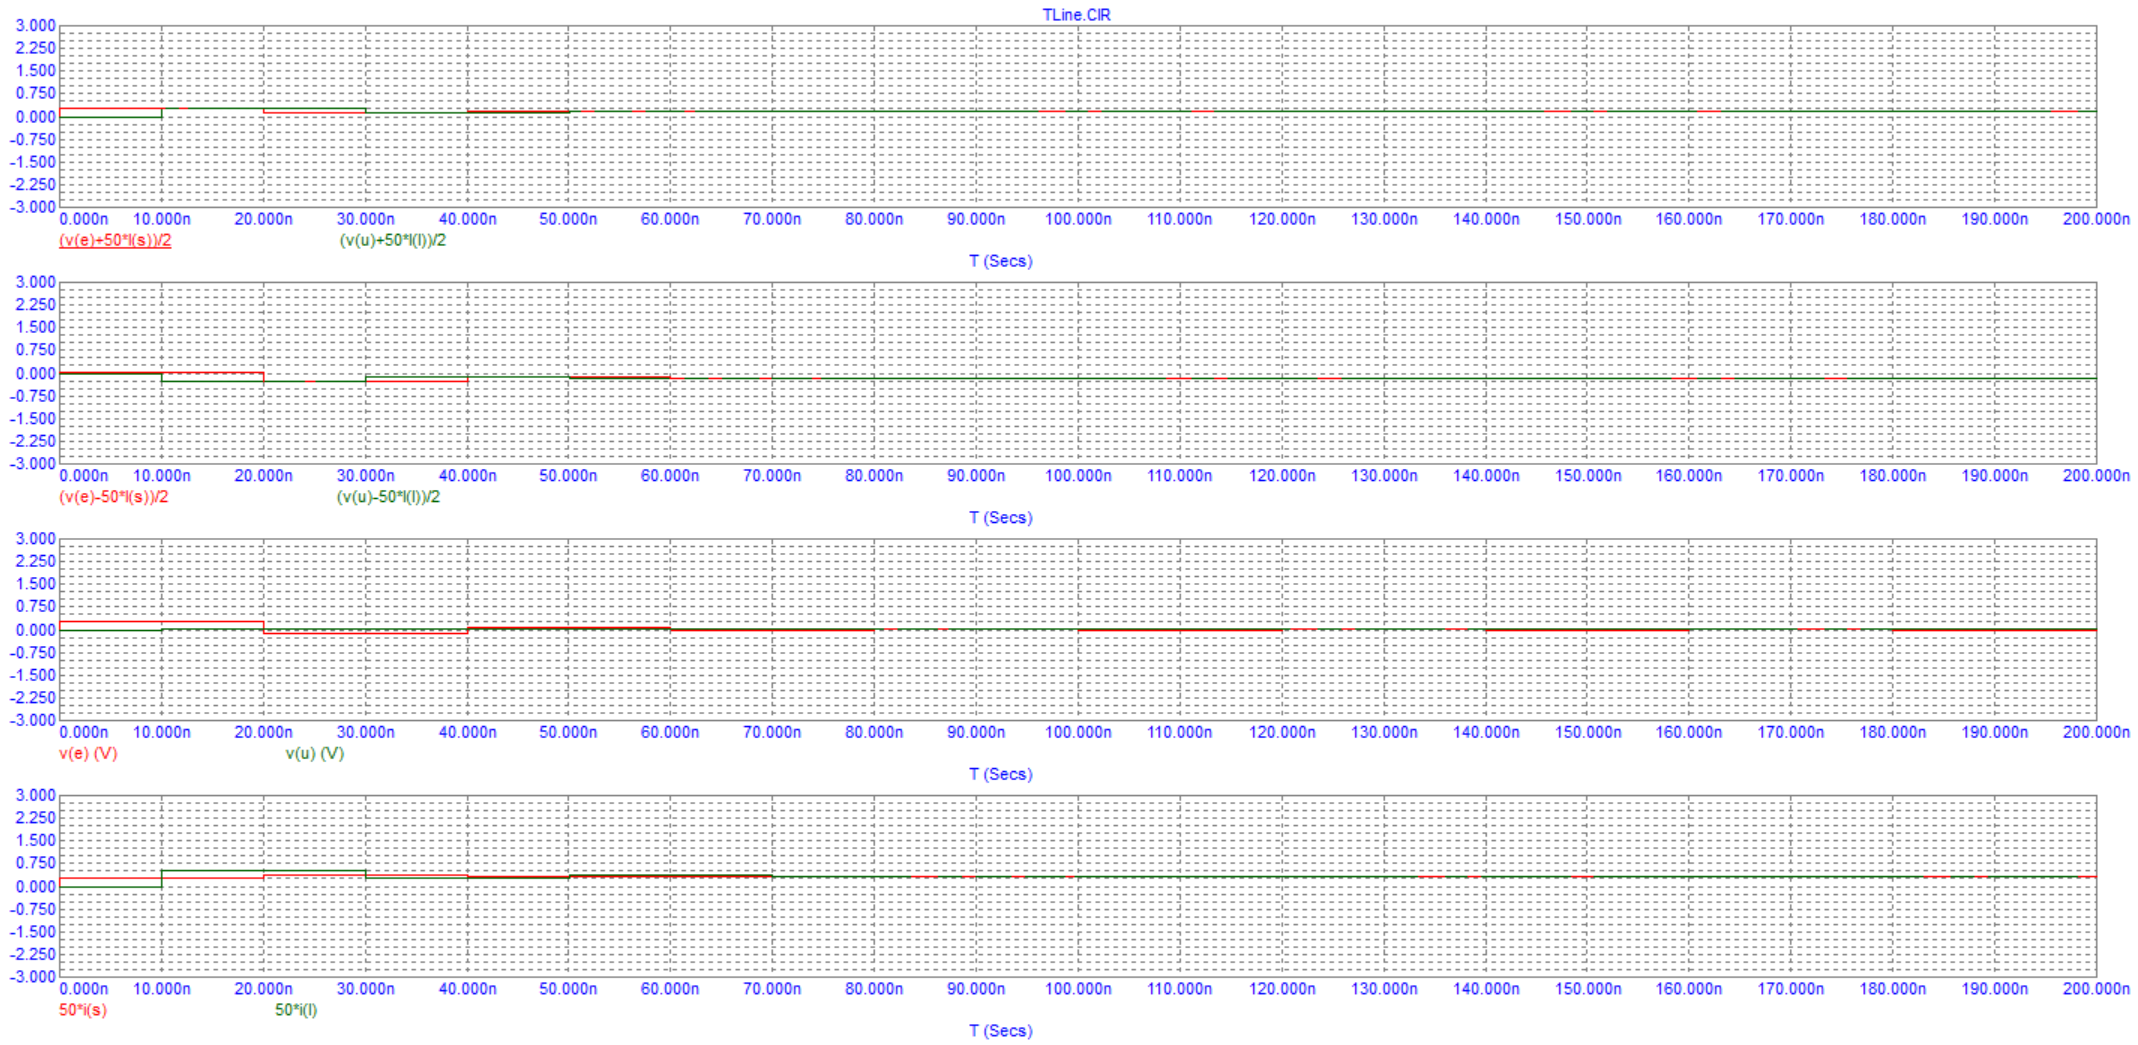
\includegraphics[scale=0.4]{images/Graph10.png}
\label{fig:Image1}
\caption{$R_l = 50k, R_s = 50/3$}
\end{figure}

\[A = \frac{\omega}{\omega + R_s} \Big( 1 + \rho_s \rho_l + (\rho_s \rho_l)^2 + ...\Big) = \frac{1}{4} \Big( 1 - \frac{1}{2} + \frac{1}{4} - ... \Big) = \frac{1}{4} \cdot \frac{2}{3} = \frac{1}{6}\]

Первый шаг $(n = 1): \: A = 0,25$.

Второй шаг $(n = 2): \: A = 1/8$.

Третий шаг $(n = 3): \: A = 3/16$.

Установившееся значение: $(n = \infty): \: A = \frac{1}{6}$.

Установить на схеме $R_s = 0 \: [\rho_s = -1]$ (предельно сильное рассогласование на источнике) и повторить наблюдения при

\[R_l = 50k, \: [\rho_l = 1] \quad \Rightarrow A = (1 -1 +1 -...),\]

\[R_l = 500, \: [\rho_l = 0,8] \quad \Rightarrow A = (1 -\rho_l + rho_l^2 -...),\]

\[R_l = 0, \: [\rho_l = 1] \quad \Rightarrow A = (1 +1 +1 +...),\]

\[R_l = 5, \: [\rho_l = -0,8] \quad \Rightarrow A = (1 +\rho_l + rho_l^2 +...),\]

\begin{figure}[h!]
\centering
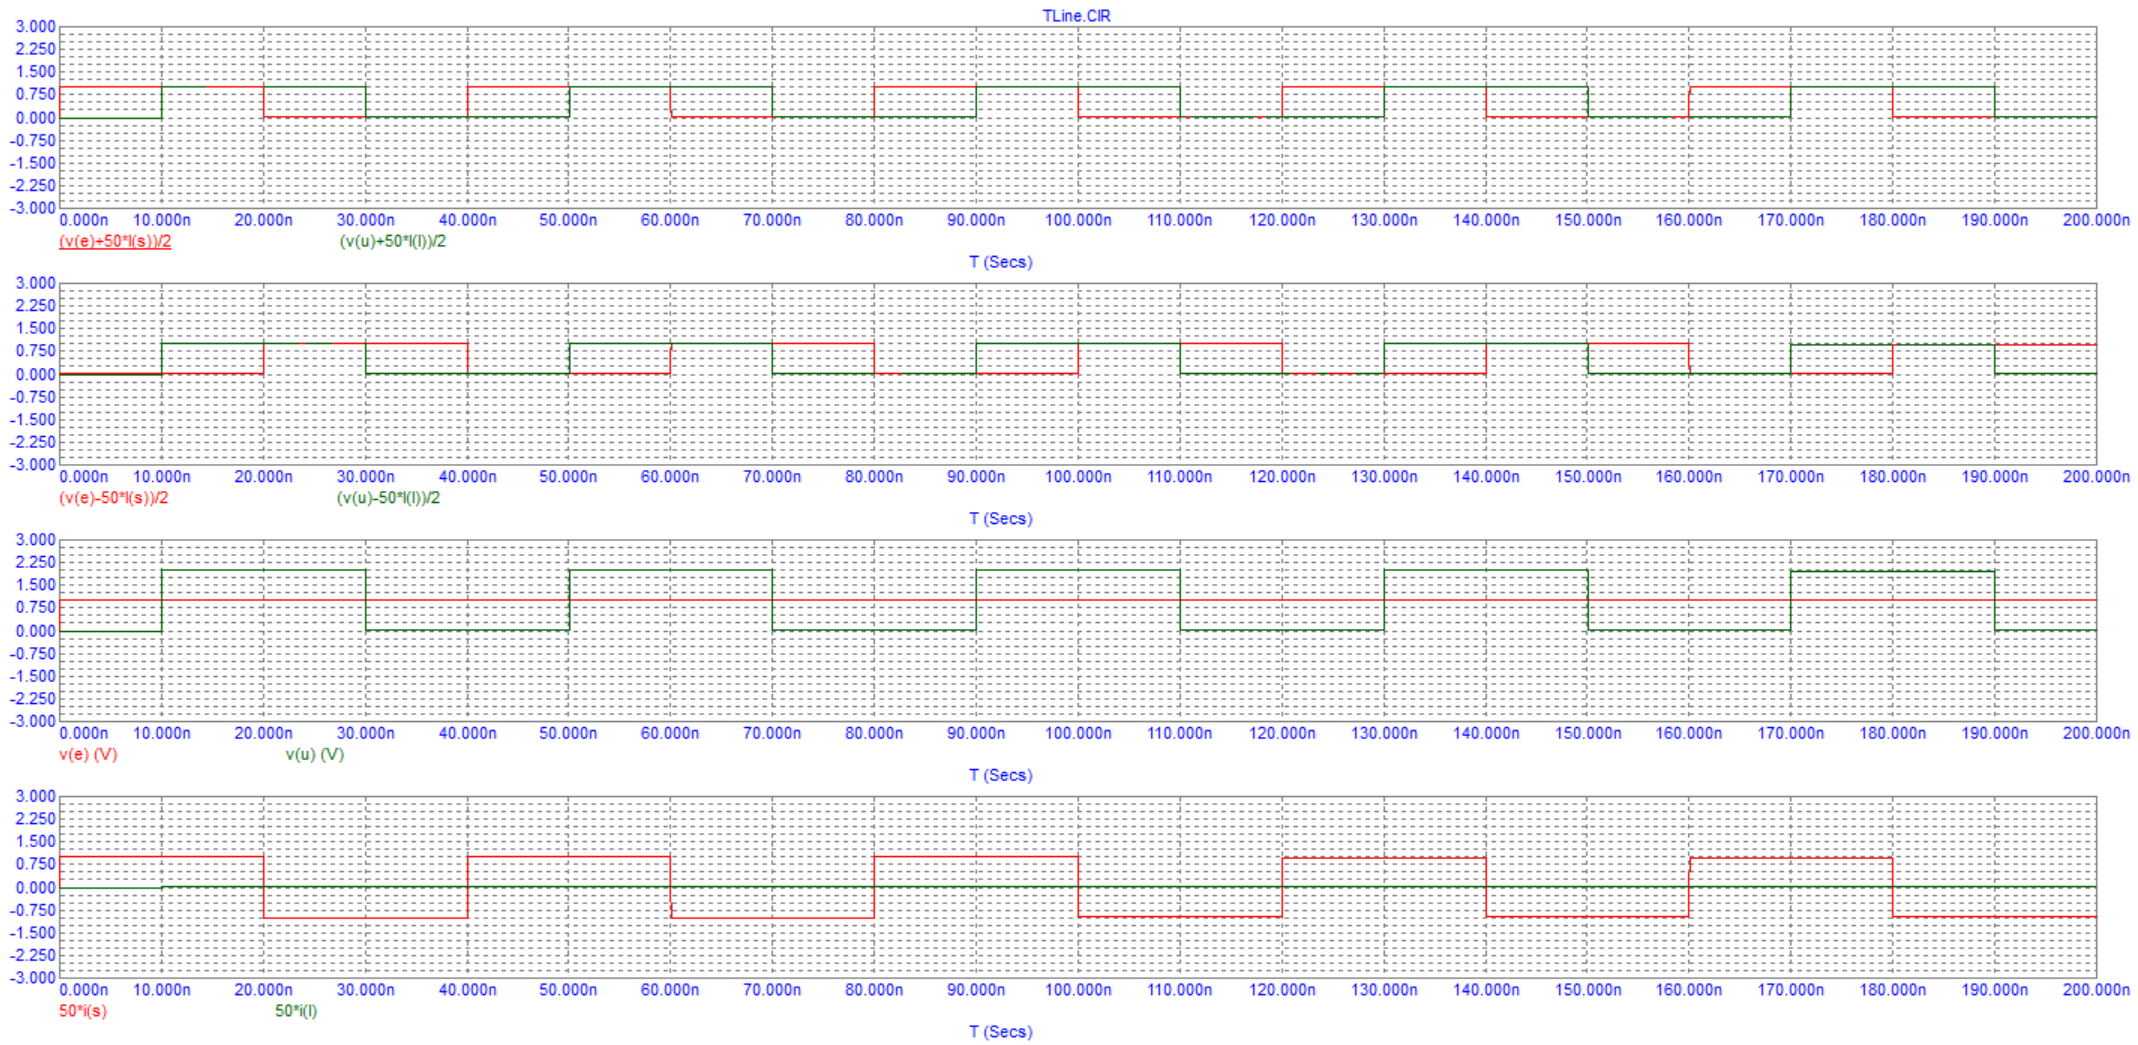
\includegraphics[scale=0.4]{images/Graph11.png}
\label{fig:Image1}
\caption{$R_l = 50k, R_s = 0$}
\end{figure}

\begin{figure}[h!]
\centering
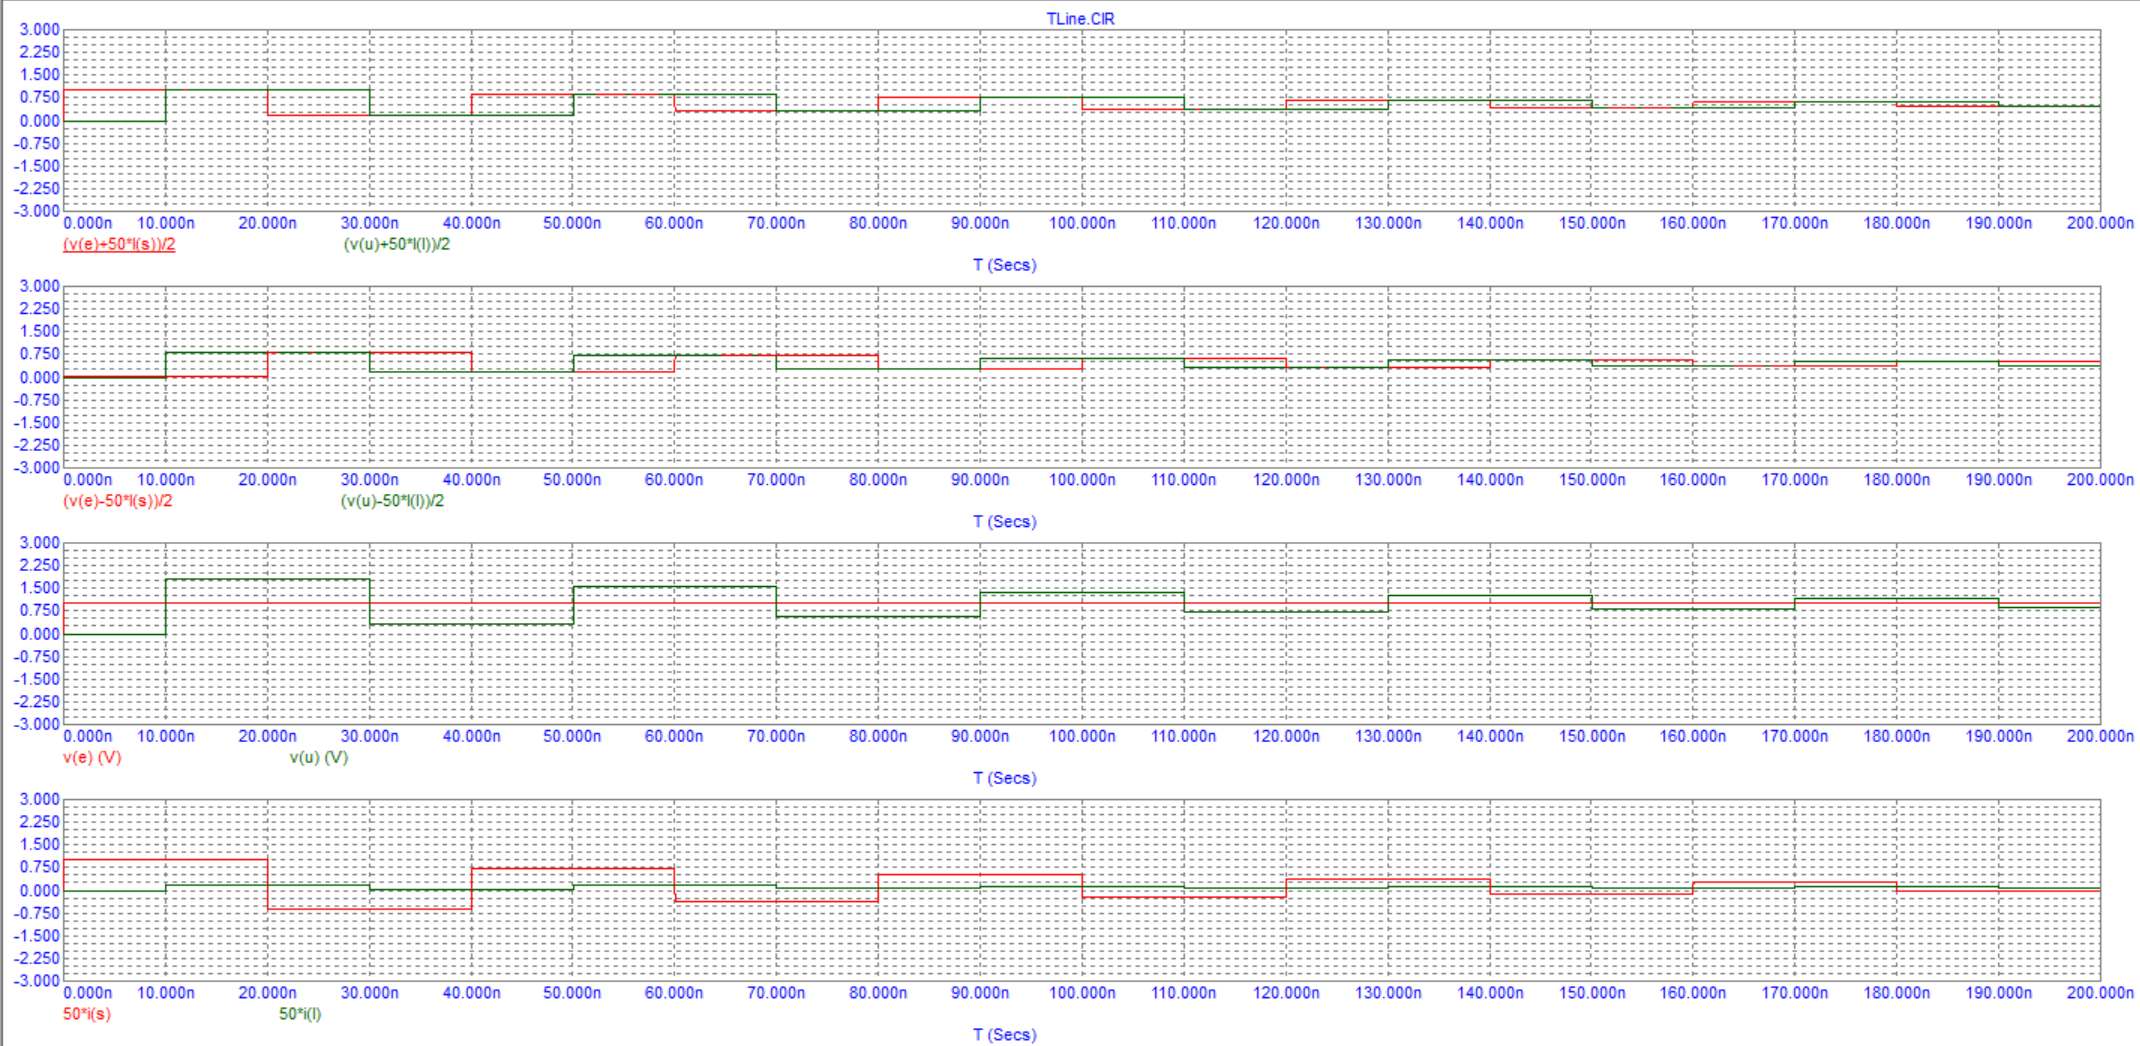
\includegraphics[scale=0.4]{images/Graph12.png}
\label{fig:Image1}
\caption{$R_l = 500, R_s = 0$}
\end{figure}

\begin{figure}[h!]
\centering
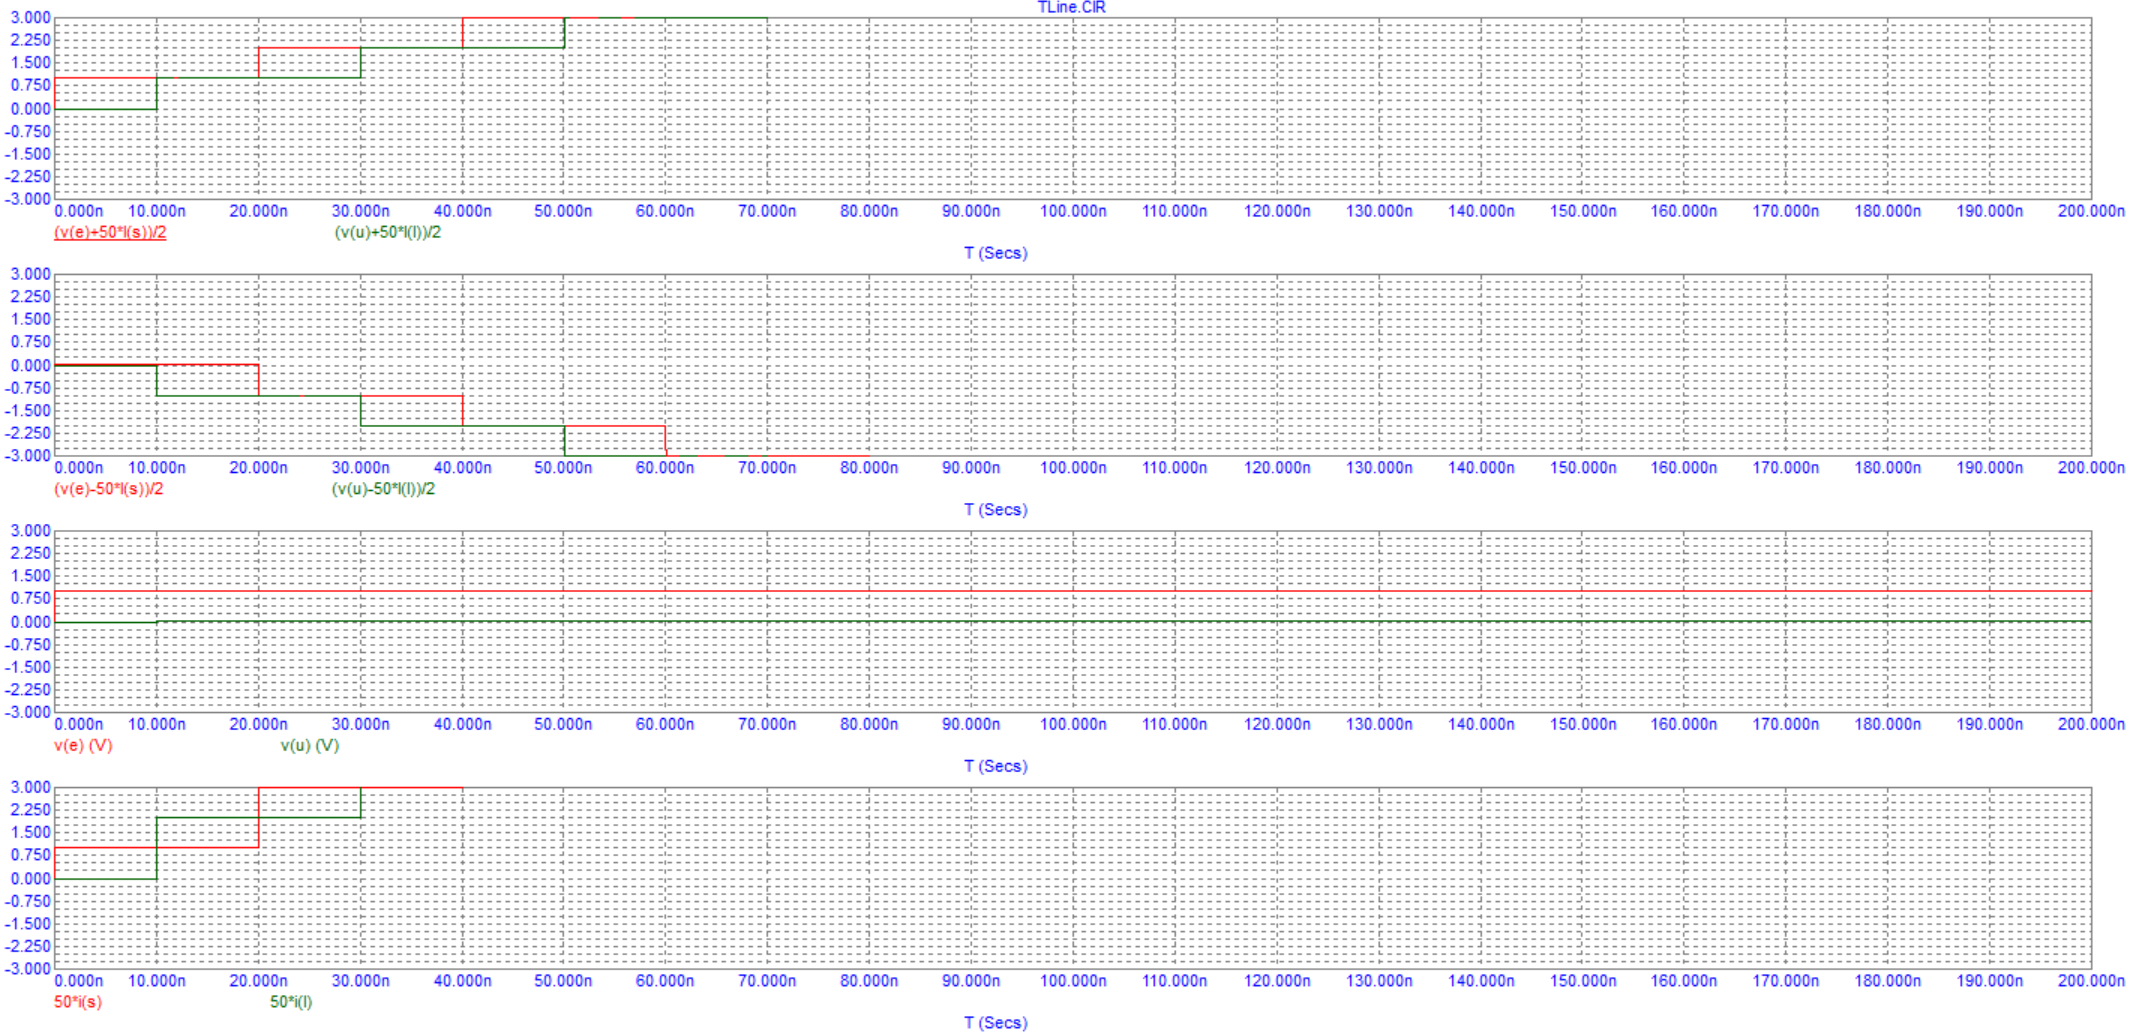
\includegraphics[scale=0.4]{images/Graph13.png}
\label{fig:Image1}
\caption{$R_l = 0, R_s = 0$}
\end{figure}

\begin{figure}[h!]
\centering
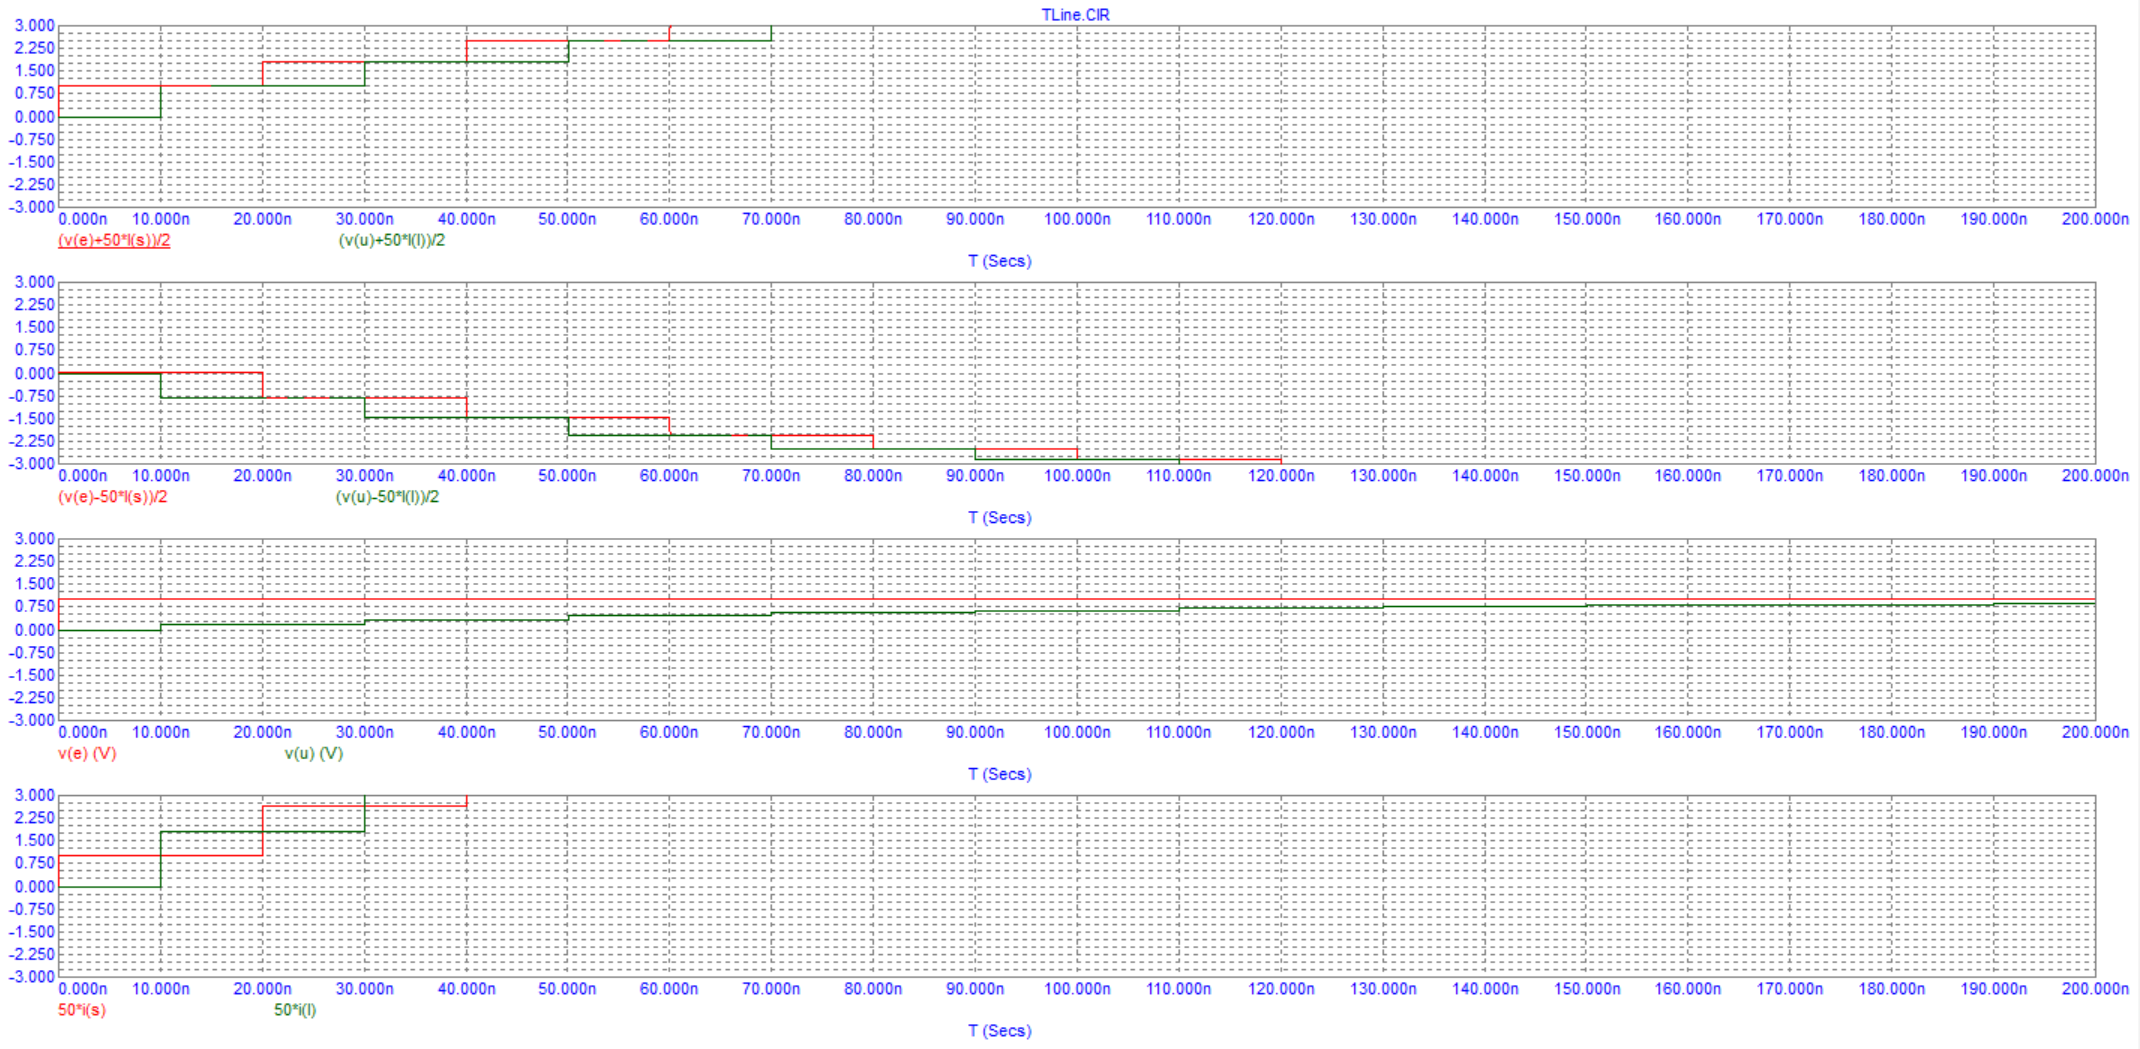
\includegraphics[scale=0.4]{images/Graph14.png}
\label{fig:Image1}
\caption{$R_l = 5, R_s = 0$}
\end{figure}

\subsection*{Емкостная нагрузка}

Установить на схеме $R_s = 50$ (согласованный источник), $R_l = 50k \simeq \infty, \: C = 100 \textit{пФ}$.

\begin{figure}[h!]
\centering
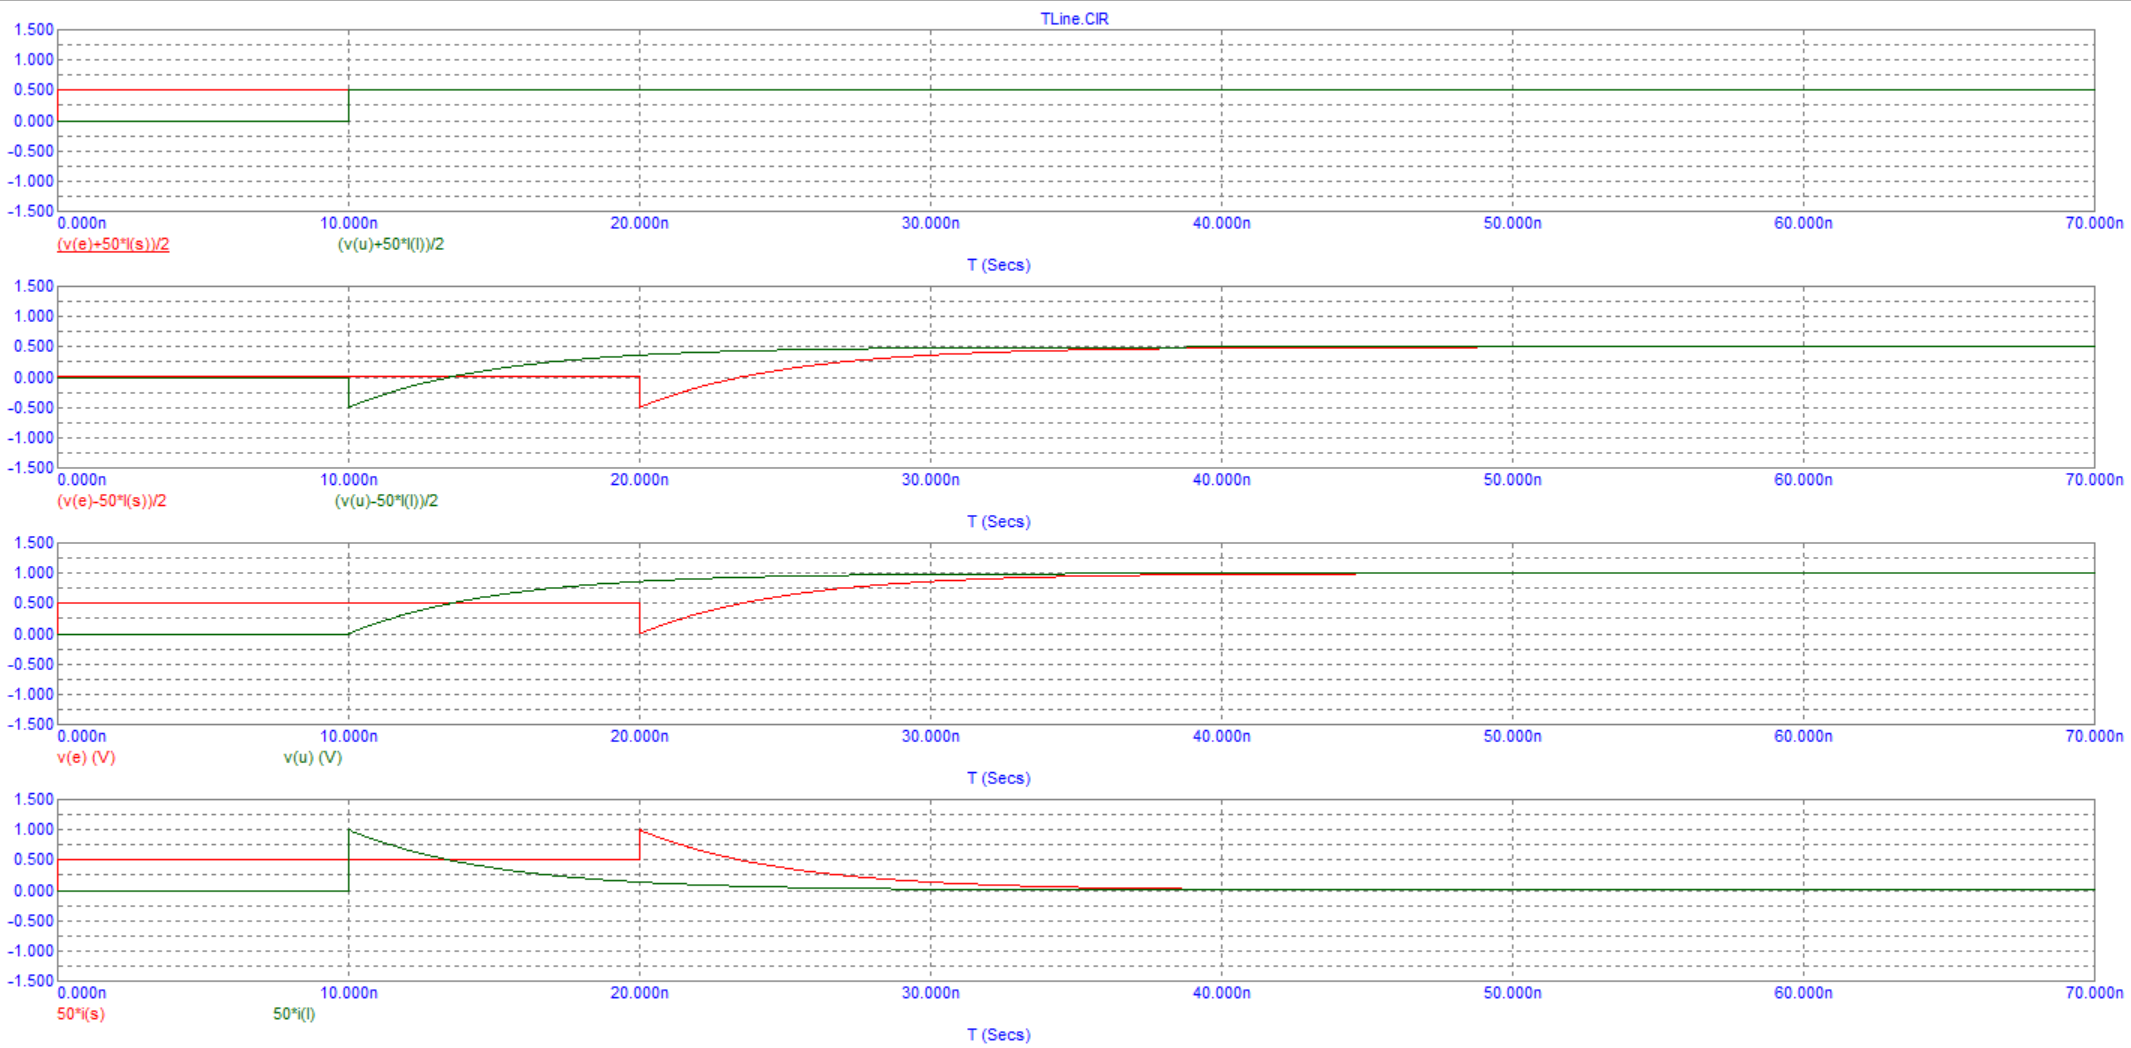
\includegraphics[scale=0.4]{images/Graph15.png}
\label{fig:Image1}
\caption{$R_l = 50k, R_s = 50$}
\end{figure}

Измерим установившееся значения амплитуд волн напряжений и токов:

\[A = 0,5 \: \textit{В}\]

\[B = 0,5 \: \textit{В}\]

\[u = 0,5 \: \textit{В}\]

\[i\omega = 0 \: \textit{В}\]

Оценим по графику постоянную времени $\tau$ экспоненциального переходного процесса:

\[u = u_0 (1 - \frac{1}{e},\]

где $u_0 = 1 \: \textit{В} \: \Rightarrow \: u = 0,63 \textit{В}$, тогда:

\[\tau_{эксп} = 5,1 \: \textit{нс}\]

\[\tau_{теор} = \omega C = 5 \: \textit{нс}\]

Варьированием установим $R_s = 50/3$, проанализируем графики переходных процессов.

\begin{figure}[h!]
\centering
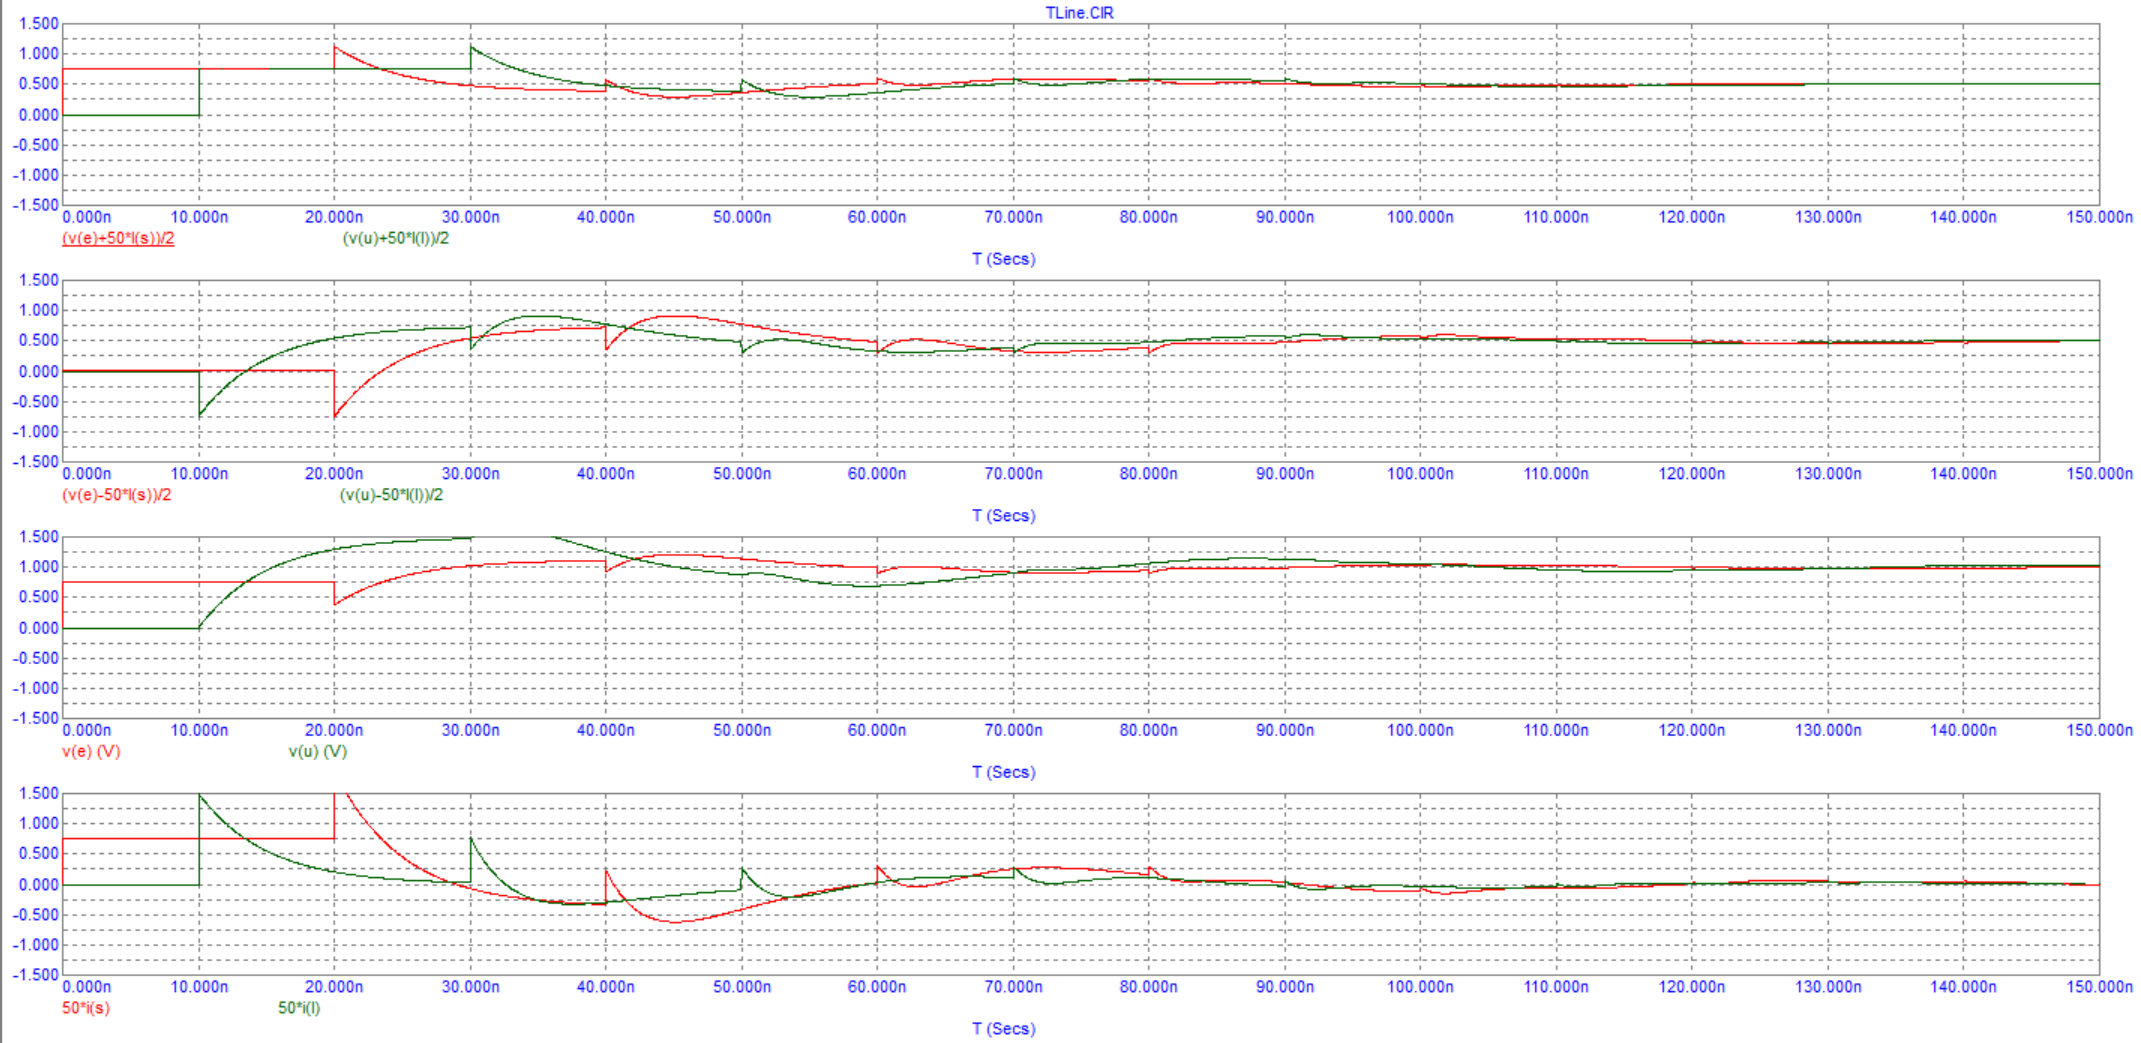
\includegraphics[scale=0.4]{images/Graph16.png}
\label{fig:Image1}
\caption{$R_l = 50k, R_s = 50/3$}
\end{figure}

\[A = 0,5 \: \textit{В}\]

\[B = 0,5 \: \textit{В}\]

\[u = 1 \: \textit{В}\]

\[i\omega = 0 \: \textit{В}\]

Проанализируем графики незатухающего переходного процесса при $R_s = 0$.

\begin{figure}[h!]
\centering
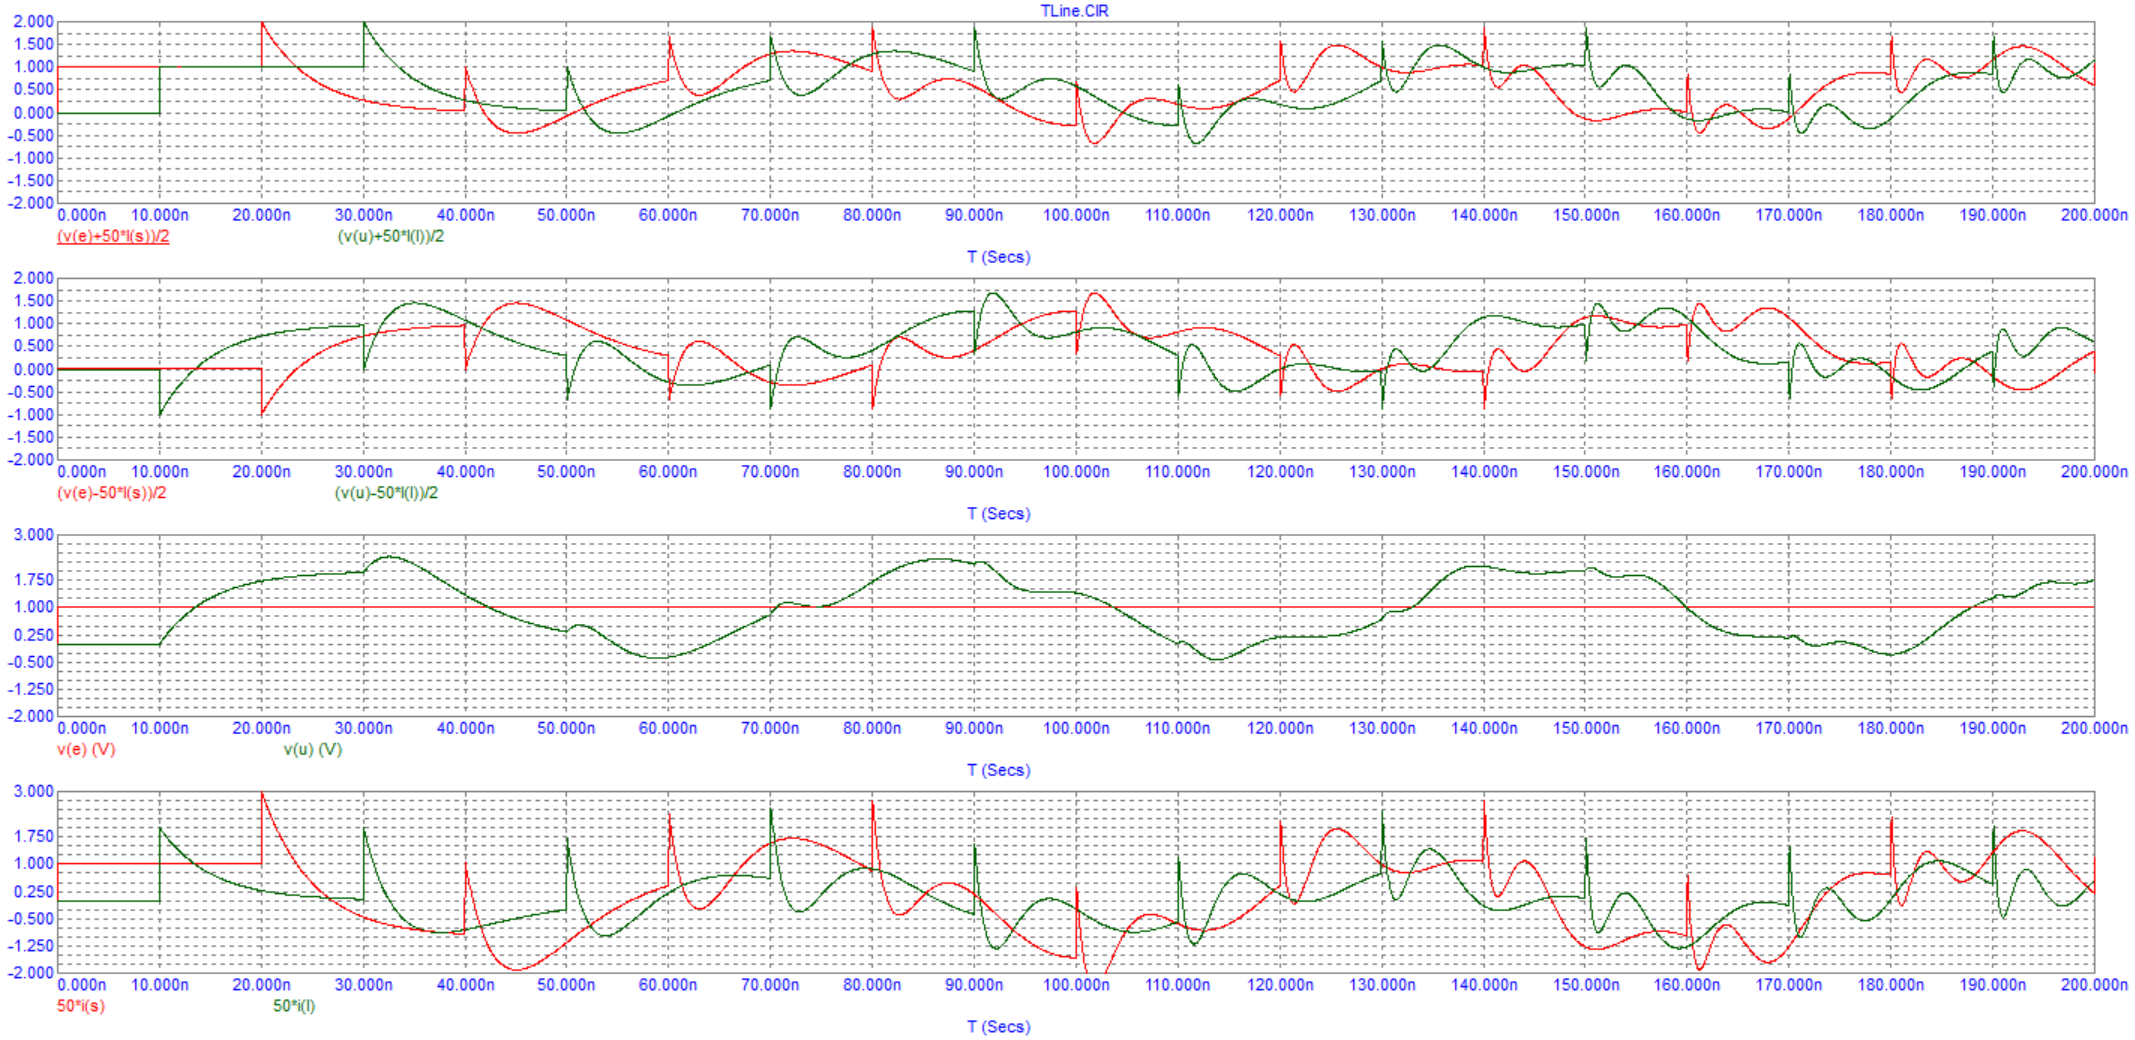
\includegraphics[scale=0.4]{images/Graph17.png}
\label{fig:Image1}
\caption{$R_l = 50k, R_s = 0$}
\end{figure}

\end{document}